\documentclass{beamer}
\usepackage[english,russian]{babel}
\usepackage[utf8]{inputenc}
% Стиль презентации
%\usetheme{Warsaw}
% \usetheme{Madrid}
%\usetheme{Marburg}
\usetheme{Hannover}

%biblatex-gost
\usepackage[backend=biber, style=gost-authoryear, language=auto, babel=other, bibencoding=utf8, bibdoi=false, biburl=false, movenames=false]{biblatex}

\addbibresource{publications_for_disser.bib}

% в начале каждого раздела печатаем содержание с выделением текущего раздела
\AtBeginSection[]
{
  \begin{frame}<beamer>{Содержание}
    \tableofcontents[currentsection]
  \end{frame}
}




\begin{document}

\title[Поселения {\it M.~balthica} Белого и Баренцева морей]{ОРГАНИЗАЦИЯ ПОСЕЛЕНИЙ {\it Macoma~balthica}~(Linnaeus,~1758) В ГРАДИЕНТАХ КЛЮЧЕВЫХ ПЕРЕМЕННЫХ СРЕДЫ ОСУШНОЙ ЗОНЫ БЕЛОГО И БАРЕНЦЕВА МОРЕЙ}
\author[С.А.~Назарова]{София Назарова \\ \medskip
	\footnotesize{Научный руководитель: д.б.н.~Н.~В.~Максимович}}
\institute[СПбГУ]{Санкт-Петербургский государственный университет}
\date{Санкт-Петербург, 2014} 
% Создание заглавной страницы
\frame{\titlepage} 





% Автоматическая генерация содержания
\frame{\frametitle{Содержание}\tableofcontents} 

		\section{Введение}

\begin{frame}{Вид {\it Macoma~balthica}}
	\begin{minipage}[b]{.39\linewidth}
		\begin{center}
			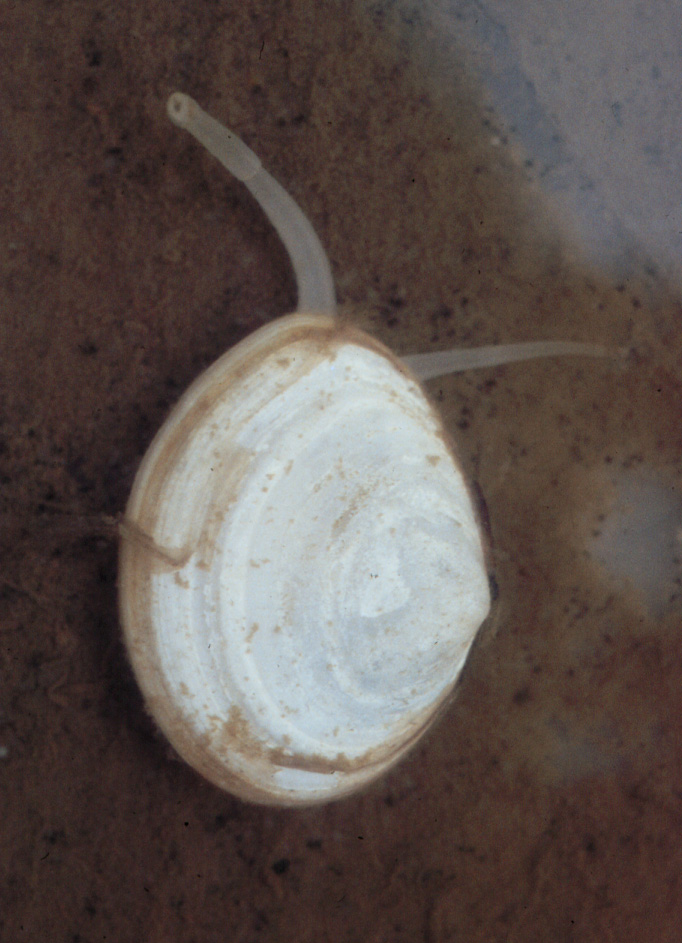
\includegraphics[width=.9\textwidth]{Macoma_balthica.jpg}
		\end{center}
	\end{minipage}
	\begin{minipage}[b]{.49\linewidth}
{\it Macoma balthica} (L.,~1758)
		\begin{itemize}
			\item{Широко распространен}
			\item{Модельный объект популяционных исследований}
			\item{Легко доступен для изучения}
			\item{Важный элемент трофических цепей}
		%	\item{}
		\end{itemize}
	\end{minipage}
\end{frame}

\begin{frame}{Цели и задачи}
\begin{description}
	\item[Цель] Изучение гетерогенности поселений {\it Macoma balthica} в условиях арктических морей.

	\item[Задачи]  Изучение:
		\begin{enumerate}
	    \item структуры сообществ макробентоса в изучаемых биотопах
	    \item структурных характеристик поселения маком: численность, биомасса, размерная структура
	    \item микрораспределения особей в поселении
	    \item показателей линейного роста маком
	    \item многолетней динамики поселений маком
	%    \item изучение абиотических характеристик местообитаний (температура, соленость, осушка, грунт);
	    \item численности спата
		  \end{enumerate}
\end{description}
\end{frame}

		\section[География]{География исследований}

\begin{frame}{Белое море}
 \begin{center}
	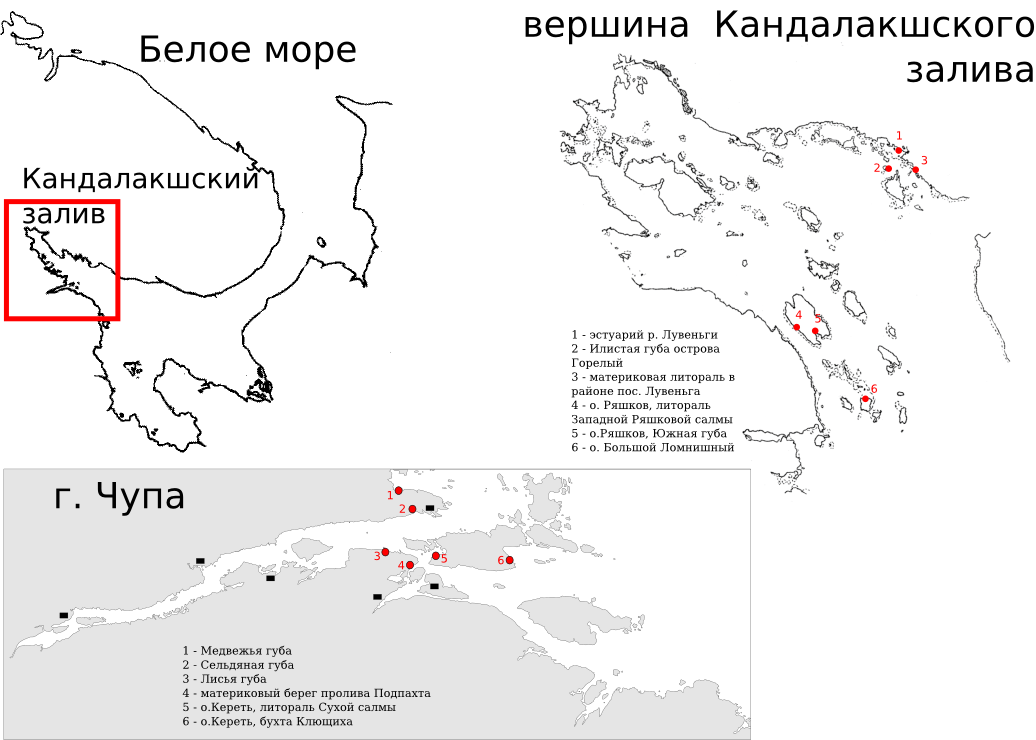
\includegraphics[width=\textwidth]{./White_Sea_map.png}
 \end{center}
\end{frame}

\begin{frame}{Баренцево море}
 \begin{center}
	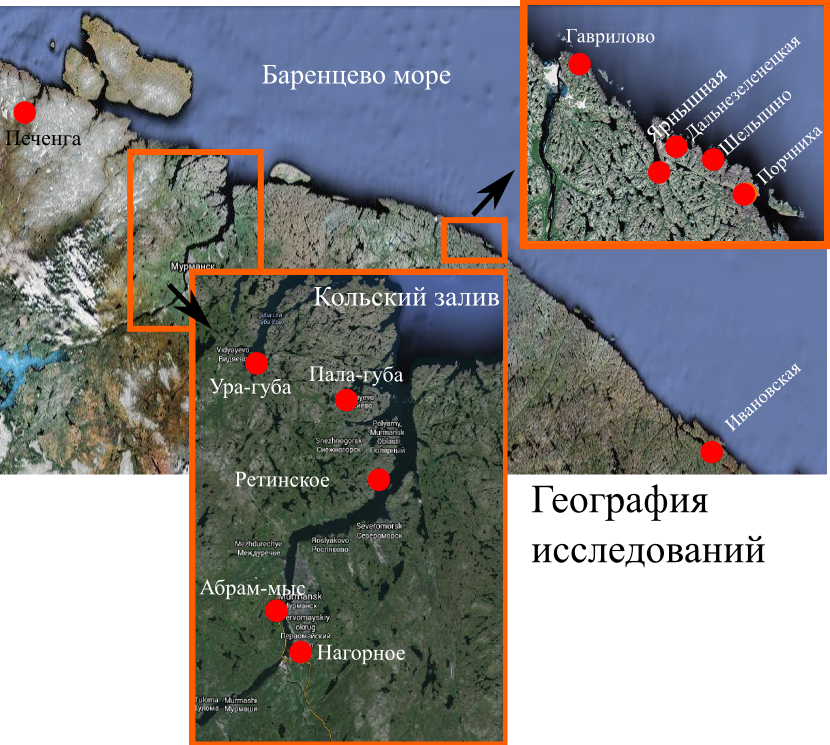
\includegraphics[width=0.85\textwidth]{./Murman_google.png}
 \end{center}
\end{frame}

%		\section[Районы исследования]{Характеристика районов исследований}
%% сделать что ли пару слайдов с фотками??
%\begin{frame}{Белое море}
% \begin{center}
%
% \end{center}
%\end{frame}
%
%\begin{frame}{Баренцево море}
% \begin{center}
%
% \end{center}
%\end{frame}

% сделать круговые диаграммы на карте с Белым и Баренцевым
%\begin{frame}{Анализ грунтов}
% \begin{center}
%
% \end{center}
%\end{frame}


		\section[Сообщество]{Таксономический состав сообществ}
\begin{frame}{Материал и методы: сообщество}
 \begin{itemize}
	\item Белое море: 6 участков, 12 описаний
	\item Баренцево море: 8 участков, 16 описаний
	\item Качественный состав сообщества
	\item Мера сходства: коэффициент Жаккара
	\item Кластеризация методом ближайшего соседа
	\item Достоверность кластеров: анализ сходства профилей (SIMPROF) (Clarke et al,2008)
 \end{itemize}
\end{frame}

% сделать круговые диаграммы на карте с Белым и Баренцевым или просто сводки по морям?
\begin{frame}{Таксономический состав}
	\begin{minipage}[b]{.49\linewidth}
		Белое море
		\begin{enumerate}
			\item Polychaeta 22
			\item Gastropoda 9
			\item Amphipoda 8
			\item Oligochaeta 5
			\item Bivalvia 4
			\item Priapulida 2
			\item Diptera 2
			\item Cumacea 2
			\item Nemertini 1
			\item Isopoda 1
			\item Decapoda 1
		\end{enumerate}
	\end{minipage}
%
	\begin{minipage}[b]{.49\linewidth}
		Баренцево море
		\begin{enumerate}
			\item Polychaeta 17
			\item Oligochaeta 8
			\item Gastropoda 6
			\item Bivalvia 5
			\item Nemertini 4
			\item Amphipoda 3
			\item Turbellaria 1
			\item Priapulida 1
			\item Diptera 1
			\item Isopoda 1
			\item Decapoda 1
		\end{enumerate}
	\end{minipage}
\end{frame}

\begin{frame}{Сравнение участков: Белое море}
	\begin{minipage}[b]{.70\linewidth}
		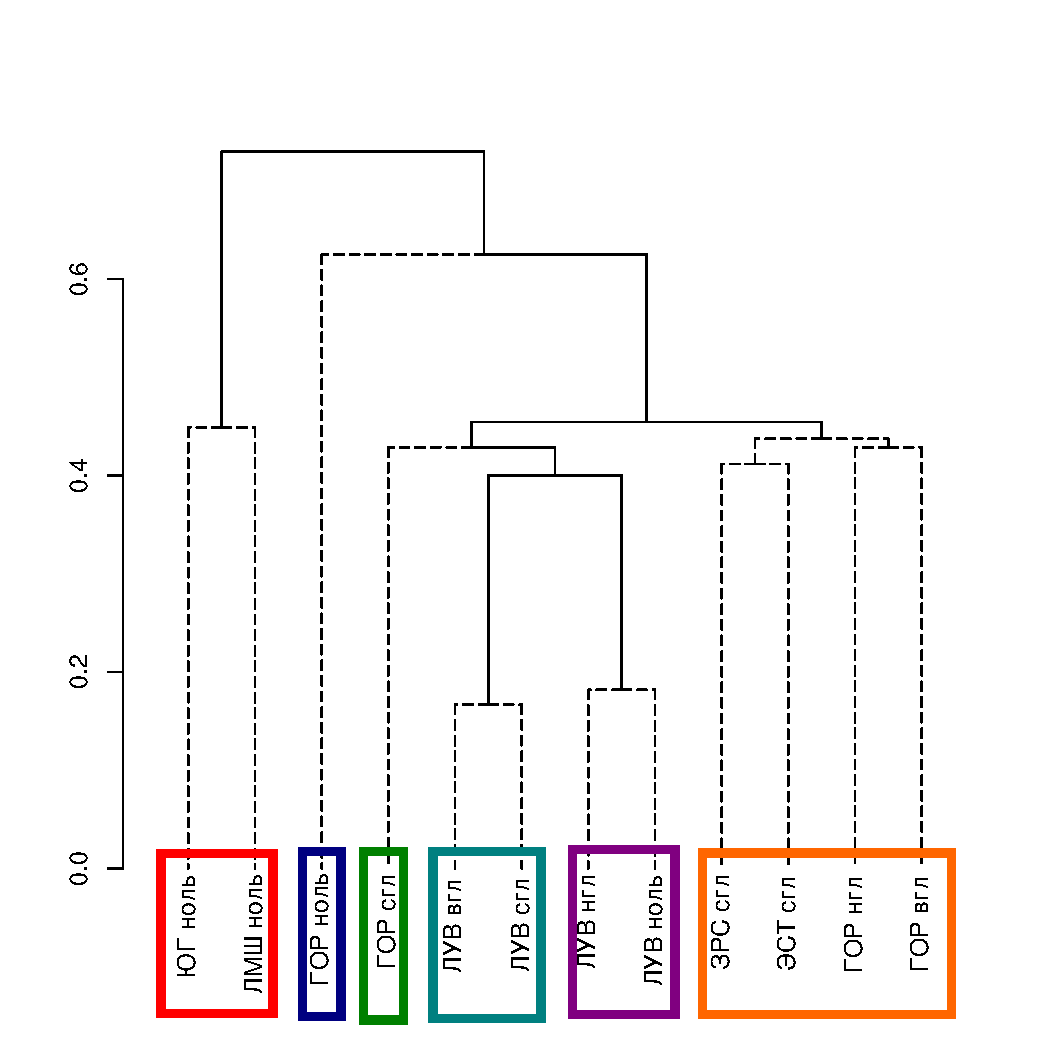
\includegraphics[width=\textwidth]{./White_fauna_tidal_jaccard_single_BW_1.pdf}
	\end{minipage}
\hfill
	\begin{minipage}[b]{.24\linewidth}
		\begin{tiny}
		ЮГ -- Южная губа о. Ряшкова \\
		ЛМШ -- о. Ломнишный \\
		ГОР -- о. Горелый \\
		ЛУВ -- материк (Лувеньга) \\
		ЭСТ -- эстуарий р. Лувеньги \\
		ЗРС -- Западная Ряшкова салма \\
		\end{tiny}
	\end{minipage}
\end{frame}

\begin{frame}{Сравнение участков: Баренцево море}
	\begin{minipage}[b]{.70\linewidth}
		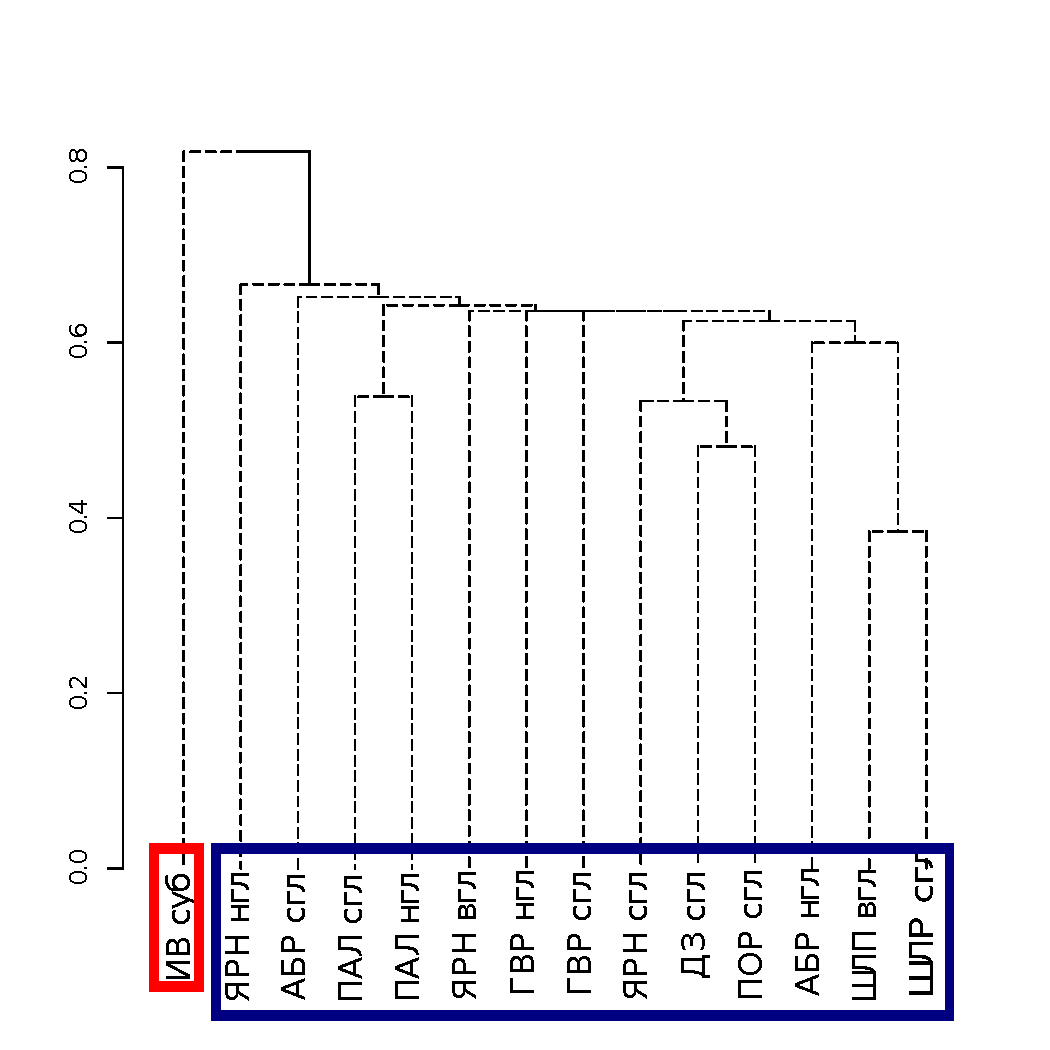
\includegraphics[width=\textwidth]{./Barents_fauna_tidal_jaccard_single_BW_1.pdf}
	\end{minipage}
\hfill
	\begin{minipage}[b]{.24\linewidth}
		\begin{tiny}
		АБР -- Абрам-мыс \\
		ПАЛ -- Пала-губа \\
		ГВР -- Гаврилово \\
		ЯРН -- Ярнышная \\
		ДЗ -- Даль\-не\-зе\-ле\-нец\-кая \\		
		ШЛП -- Шельпино \\
		ПОР -- Порчниха \\
		ИВ -- Ивановская \\
		\end{tiny}
	\end{minipage}

\end{frame}

\begin{frame}{Основные результаты: сообщество}
 \begin{itemize}
	\item Белое море: 57 таксонов, преобладают Polychaeta
	\item Сходство фаун в поселениях маком Кандалакшского залива определяется как мареографическим уровнем, так и географической близостью участков
	\item Баренцево море: 48 таксонов, преобладают Polychaeta
	\item В пределах литорали фауна в поселениях  маком Мурманского побережья Баренцева моря не различается достоверно между горизонтами литорали и исследованными участками
 \end{itemize}
\end{frame}

		\section[Мик\-ро\-рас\-пре\-де\-ле\-ние]{Микрораспределение {\it Macoma balthica}}
\begin{frame}{Материал и методы: распределение}
\begin{itemize}
	\item Баренцево море: Дальнезеленецкая (2007, 2008), Ярнышная (2008), Пала-губа (2008)
	\item масштабированная схема из Trush et al., 1989
	\item полигон $7,5 \times 12$~ м, 12 секторов внутри полигона
	\item случайное расположение 3 проб площадью 1/30~м$^2$ внутри сектора
	\item фиксация коорднат проб относительно краев полигона
	\item всего 36 проб 
	\item промывка на сите 1~мм
	\item Статистика: пространственные автокореляции Морана, корреляции Кендалла
\end{itemize}
\end{frame}

% тут надо сделать схемы про распределение
\begin{frame}{Ярнышная: нет паттерна}
	\begin{minipage}[t]{.7\linewidth}
 \begin{center}
		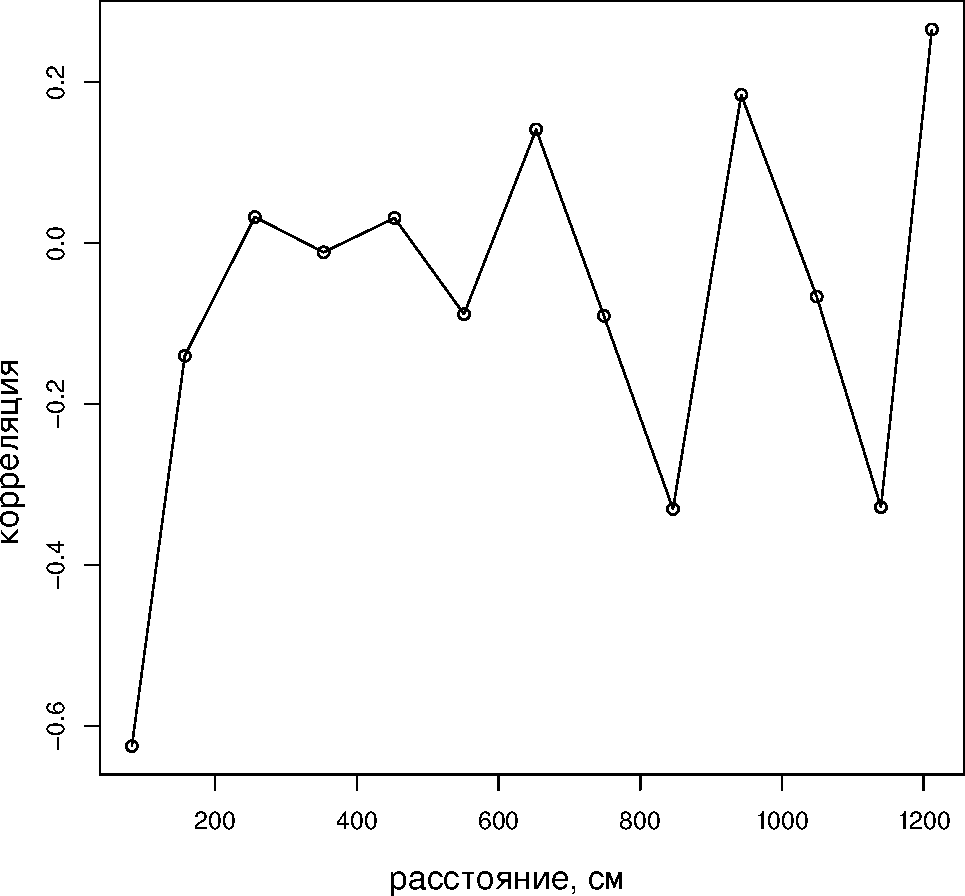
\includegraphics[width=\textwidth]{Yarnyshnaya07_moran_N_Macoma_balthica_.pdf}
 \end{center}
	\end{minipage}
	\begin{minipage}[t]{.28\linewidth}
 \begin{center}
		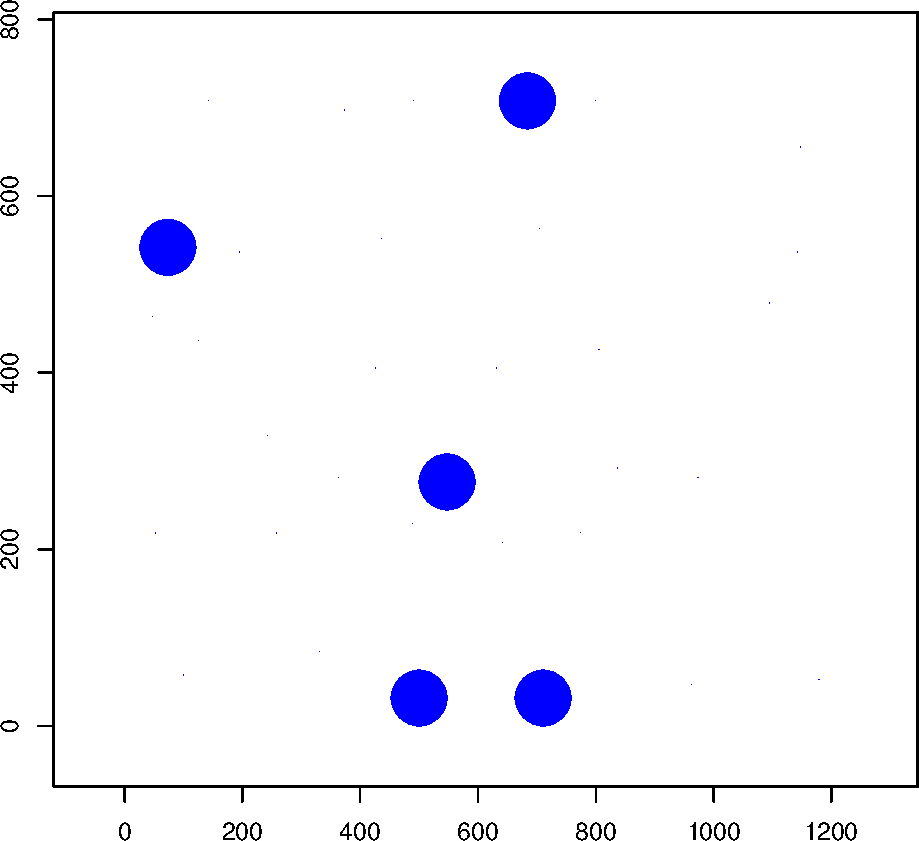
\includegraphics[width=\textwidth]{Yarnyshnaya_N_cockle_bubbles.pdf}
 \end{center}
	\end{minipage}
\end{frame}

\begin{frame}{Дальнезеленецкая: пятна агрегации}
	\begin{minipage}[t]{.7\linewidth}
 \begin{center}
		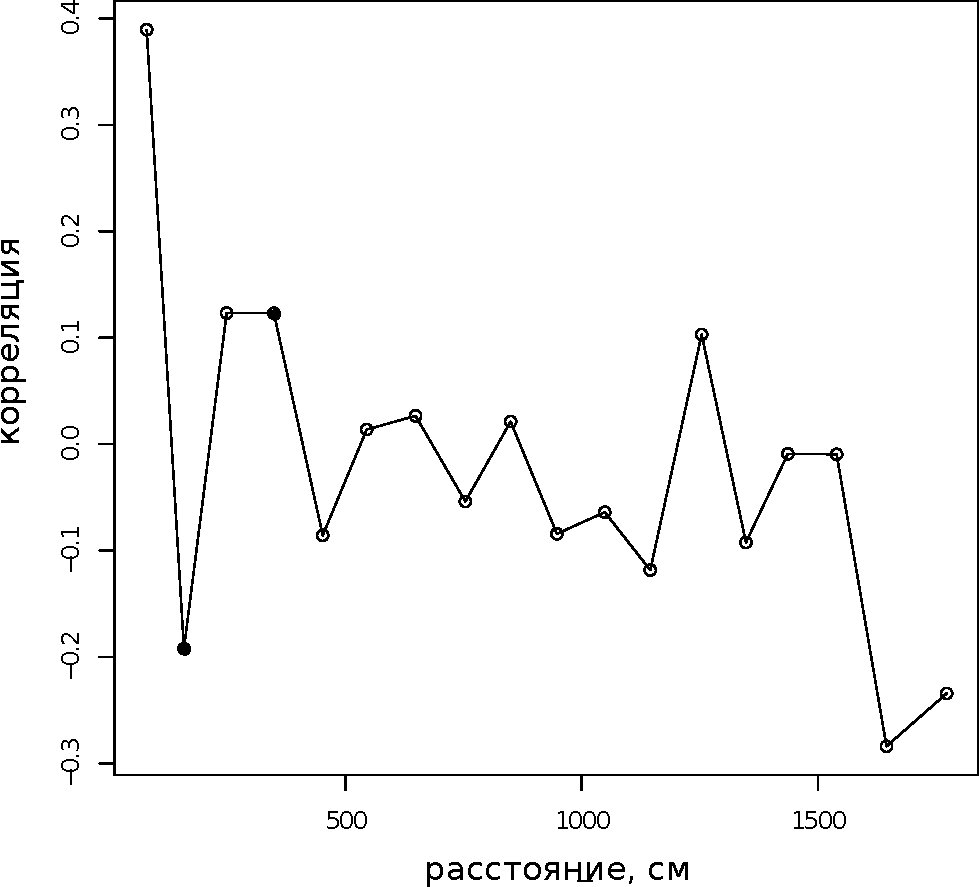
\includegraphics[width=\textwidth]{Plyazh0812_moran_N_Macoma_balthica_.pdf}
 \end{center}
	\end{minipage}
	\begin{minipage}[t]{.28\linewidth}
 \begin{center}
		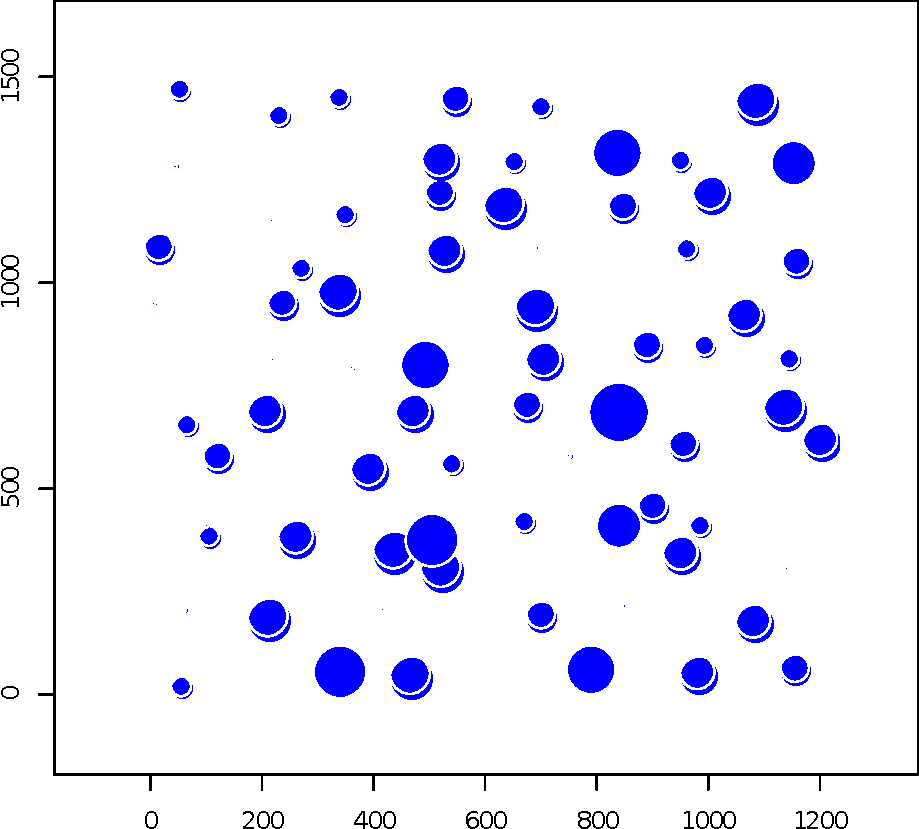
\includegraphics[width=\textwidth]{Plyazh0812_N_Macoma_bubbles.pdf}
 \end{center}
	\end{minipage}
\end{frame}


\begin{frame}{Пала-губа: градиент}
	\begin{minipage}[t]{.7\linewidth}
 \begin{center}
		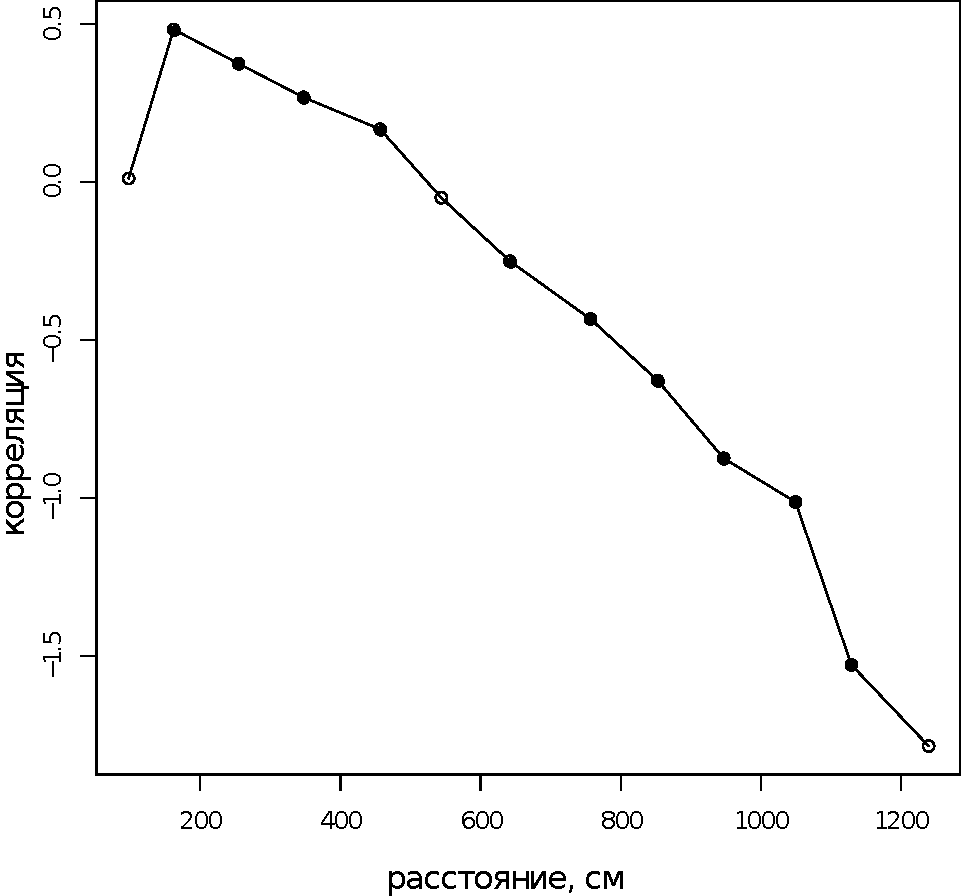
\includegraphics[width=\textwidth]{Pala_moran_N_Macoma_balthica_.pdf}
 \end{center}
	\end{minipage}
	\begin{minipage}[t]{.28\linewidth}
 \begin{center}
		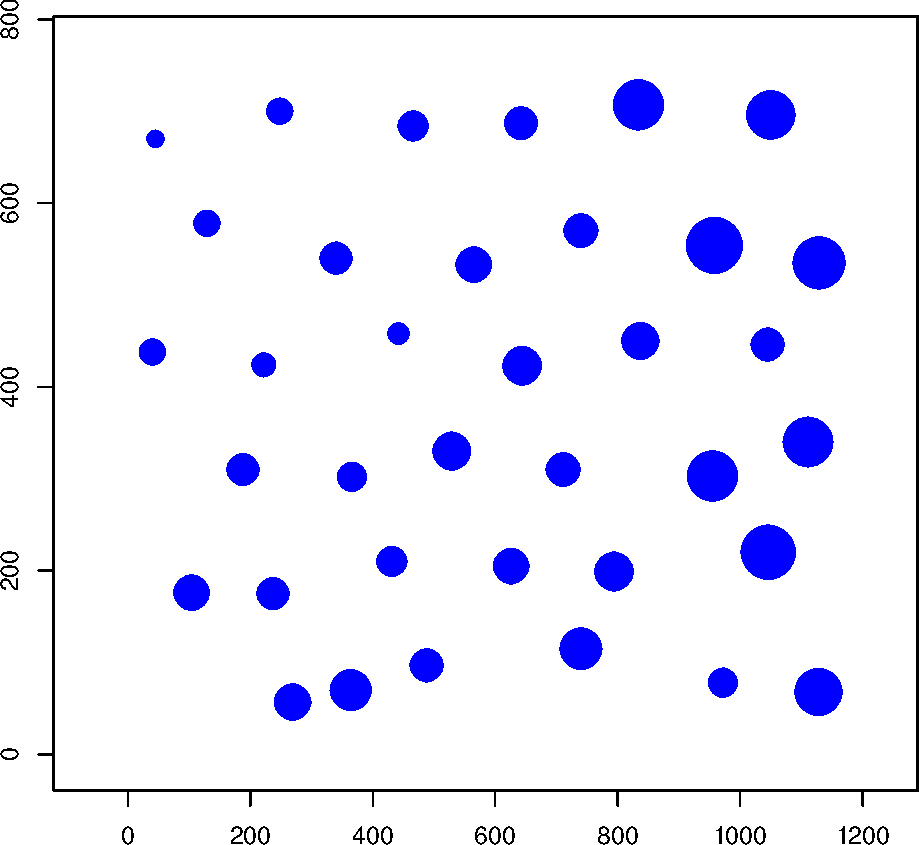
\includegraphics[width=\textwidth]{Pala_N_Macoma_bubbles.pdf}

 \end{center}
	\end{minipage}
\end{frame}

\begin{frame}{Основные результаты: распределение}
\begin{itemize}
	\item Дальнезеленецкая: скопления особей, сравнимые с размером пробы, организованные в крупные пятна размером около 4 м
	\item Пала-губа: градиент, связанный с наличием крупного ручья. 
	\item Пала-губа: различный паттерн распределения особей разных возрастов. Молодые особи тяготеют к ручью, старые организованы в пятна разного размера независимо от ручья

\end{itemize}
\end{frame}

		\section[Обилие]{Обилие {\it Macoma balthica}}
\begin{frame}{Материал и методы: обилие}
\begin{itemize}
	\item Белое море: 10 участков
	\item Баренцево море: 12 участков	
	\item Рамки площадью 1/30 и 1/20~м$^2$
	\item Сито 1 мм
	\item Число повторностей: Белое море --- $3-16$, Баренцево море --- $3-72$
	\item Биомасса: сырой вес, для части участков на Белом море --- пересчет по измеренной длине раковины (Максимович и др., 1993)

\end{itemize}
\end{frame}

\begin{frame}{Белое море: участки}
 \begin{center}
		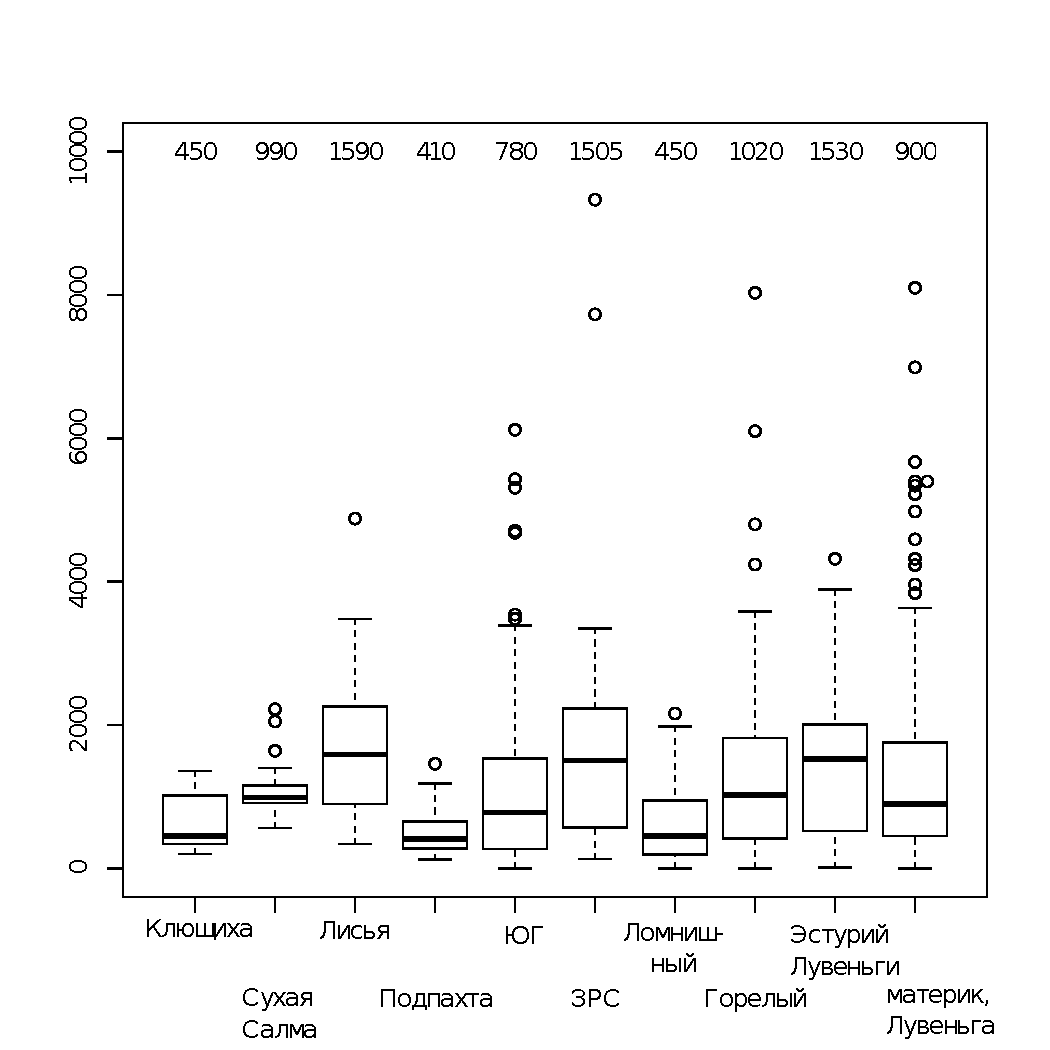
\includegraphics[width=.8\textwidth]{N2_area_White1.pdf}
 \end{center}
\end{frame}

\begin{frame}{Баренцево море: участки}
 \begin{center}
		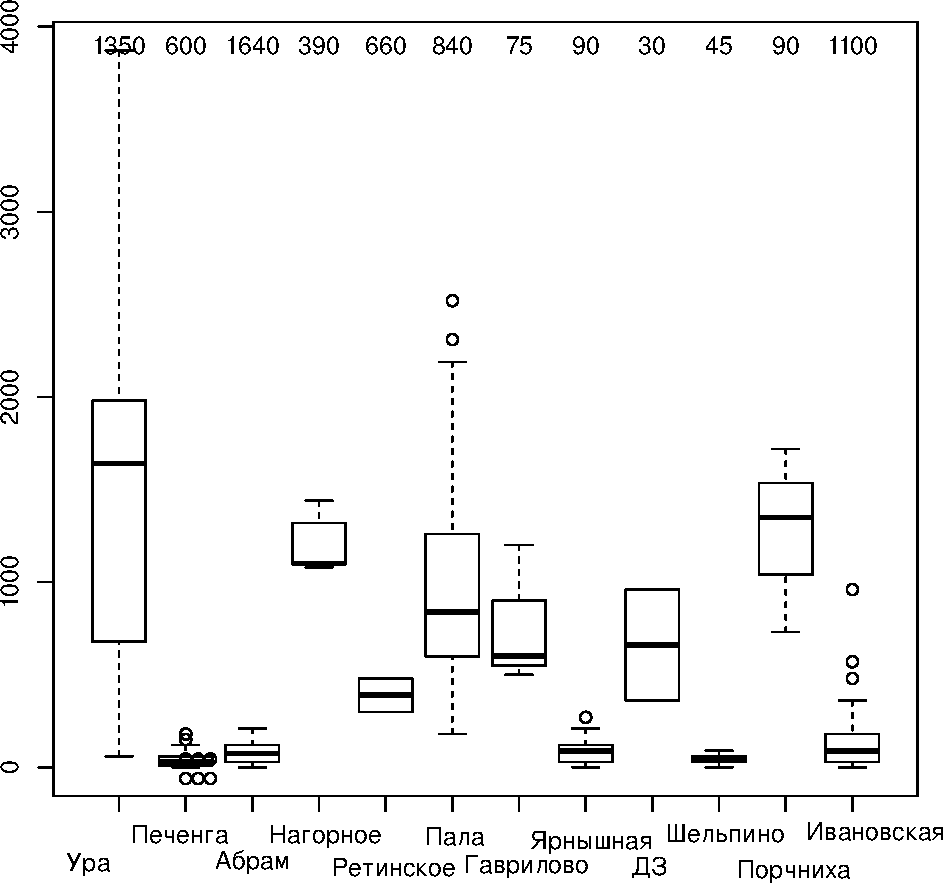
\includegraphics[width=.8\textwidth]{N2_area_Barents1.pdf}
 \end{center}
\end{frame}

\begin{frame}{Баренцево море: районы}
 \begin{center}
		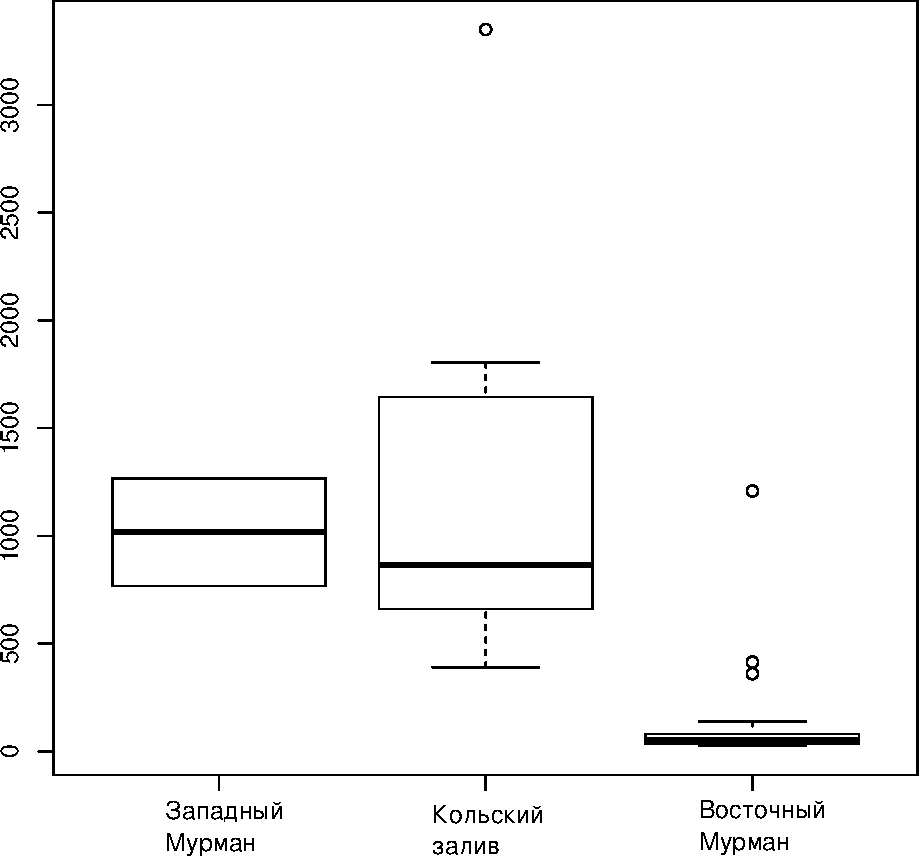
\includegraphics[width=.7\textwidth]{Nmean_region_Barents1.pdf}
 \end{center}
$Kruskal-Wallis\ \chi^2 = 17,6, p < 0,001$
\end{frame}

\begin{frame}{Обилие маком в Европейской части ареала}
 \begin{center}
		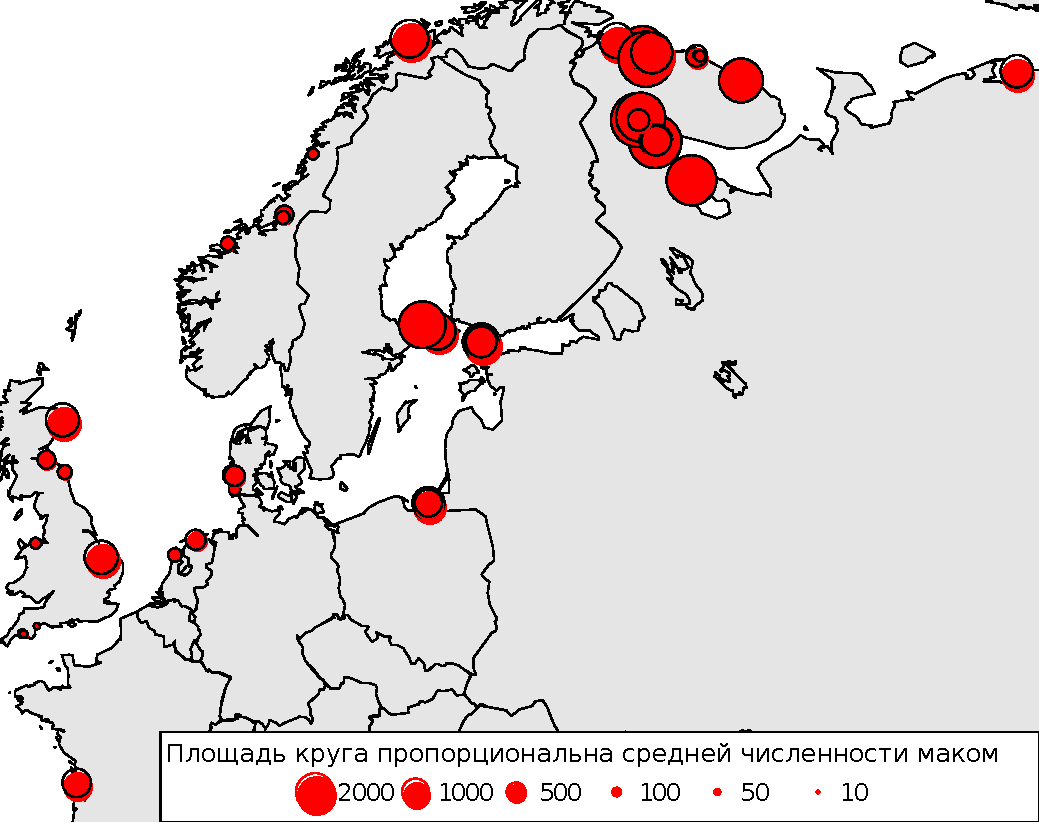
\includegraphics[width=.9\textwidth]{Nmean_1.pdf}
 \end{center}
\end{frame}


\begin{frame}{Основные результаты: обилие}
		\begin{enumerate}
			\item Средняя численность маком варьирует: в Белом море --- от 10 до 8500~экз./м$^2$, в Баренцевом --- от 30 до 3350~экз./м$^2$
			\item Средняя биомасса маком варьирует: в Белом море --- от 1 до 180~г/м$^2$,  в Баренцевом --- от 13 до 210~г/м$^2$
			\item Типичны поселения маком с обилием: в Белом море ---  700-800~экз./м$^2$, в Баренцевом --- менее 100~экз./м$^2$
			\item Отдельные районы Кандалакшского залива Белого моря не различаются по средней численности маком
			\item Численность маком на Восточном Мурмане ниже, чем на Западном и в Кольском заливе
			\item Вертикальное распределение маком различно на разных участках
			\item Среднее обилие маком в поселениях Белого моря и Кольского залива Баренцева моря выше, чем в других частях ареала. 
		\end{enumerate}
\end{frame}

		\section[Размерная структура]{Размерная структура {\it Macoma balthica}}
\begin{frame}{Материал и методы: размерная структура}
\begin{itemize}
	\item Белое море: 6 мониторинговых участков
	\item Баренцево море: 7 участков. 1 мониторинг.
	\item Рамки площадью 1/30 и 1/20~м$^2$
	\item Сито 1 мм
	\item Число повторностей: Белое море --- $3-16$, Баренцево море --- $3-72$
	\item Измерение длины раковины с точностью 0,1мм
\end{itemize}
\end{frame}

\begin{frame}{Эстуарий р.~Лувеньги:динамика с чередованием типов структур}
 \begin{center}
		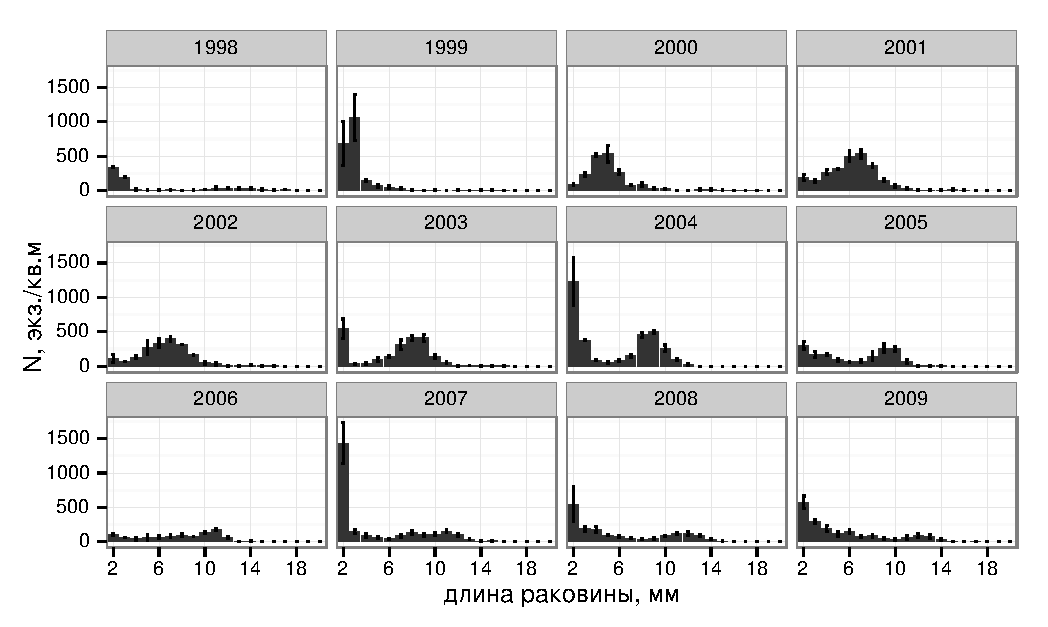
\includegraphics[width=\textwidth]{Estuary_sizestr_oneplot.pdf}
 \end{center}
\end{frame}

\begin{frame}{Южная губа о.~Ряшкова: динамика с повторением структур}
 \begin{center}
		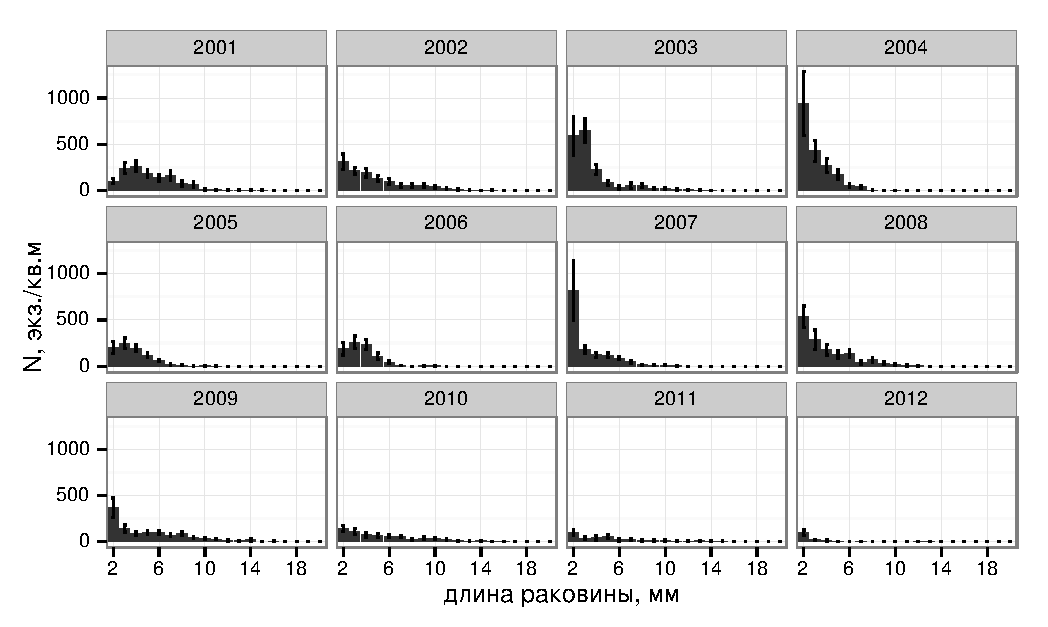
\includegraphics[width=\textwidth]{YuG_sizestr_oneplot.pdf}
 \end{center}
\end{frame}

\begin{frame}{г. Дальнезеленецкая}
 \begin{center}
		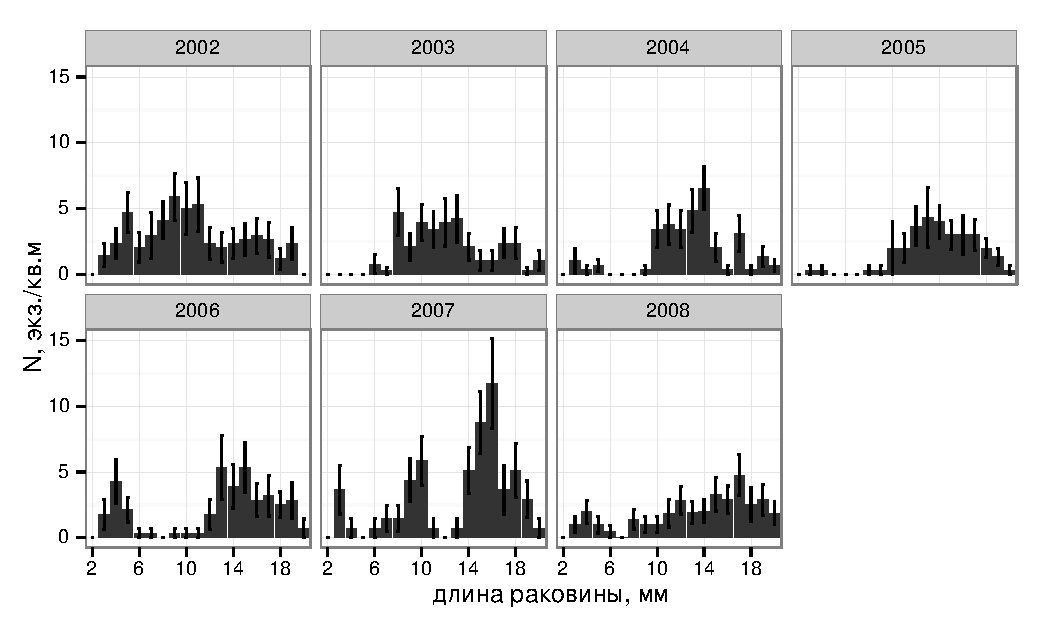
\includegraphics[width=\textwidth]{DZ_sizestr_oneplot.pdf}
 \end{center}
\end{frame}

\begin{frame}{Основные результаты: размерная структура}
	\begin{enumerate}
		\item Максимальный размер: Белое море --- 24~мм, Баренцево море --- 21~мм
		\item Тип структуры: бимодальный, несколько реже --- мономодальный (преобладают обычно молодые особи), при низкой численности может быть практически равномерное распределение.
		\item В бимодальной структуре второй модальный класс: Белое море --- обычно особи длиной 9-12 мм, Баренцево --- часто особи длиной 14-17~мм.
		\item Динамика размерной структуры: чередование бимодальной и мономодальной размерной структур. Мономодальная обычно сохраняется 1-2 года.
		\item Есть участки с ежегодно повторяющейся мономодальной размерной структурой
	\end{enumerate}
\end{frame}


		\section[Линейный рост]{Линейный рост {\it Macoma balthica}}
\begin{frame}{Материал и методы: рост}
\begin{itemize}
	\item Баренцево море: 7 участков.
	\item Кадастровая съемка $2007 - 2008$ года
	\item Измерения: длина раковины, длина меток зимних остановок роста
	\item Число меток зимних остановок роста = возраст
	\item Горизонты литорали рассматривали отдельно: всего 14 описаний роста
	\item Аппроксимация рядов: линейная модификация уравнения Берталанфи: $L_{t} = L_{max} \times (1 - e^{(-k(t - t_{0}))})$
	\item Сравнение кривых роста: сравнение остаточных дисперсий по методике Н.В.~Максимовича (1989), по параметру $\omega = k * L_{max}$ (Appeldoorn,1983)
	\item Влияние географии и мареографии на годовой прирост: дисперсионный анализ (ANOVA)
\end{itemize}
\end{frame}

\begin{frame}{Сравнение кривых роста}
	\begin{minipage}[t]{.6\linewidth}
\begin{center}
	\tiny{Линейный рост {\it Macoma balthica} в Баренцевом море}\\
			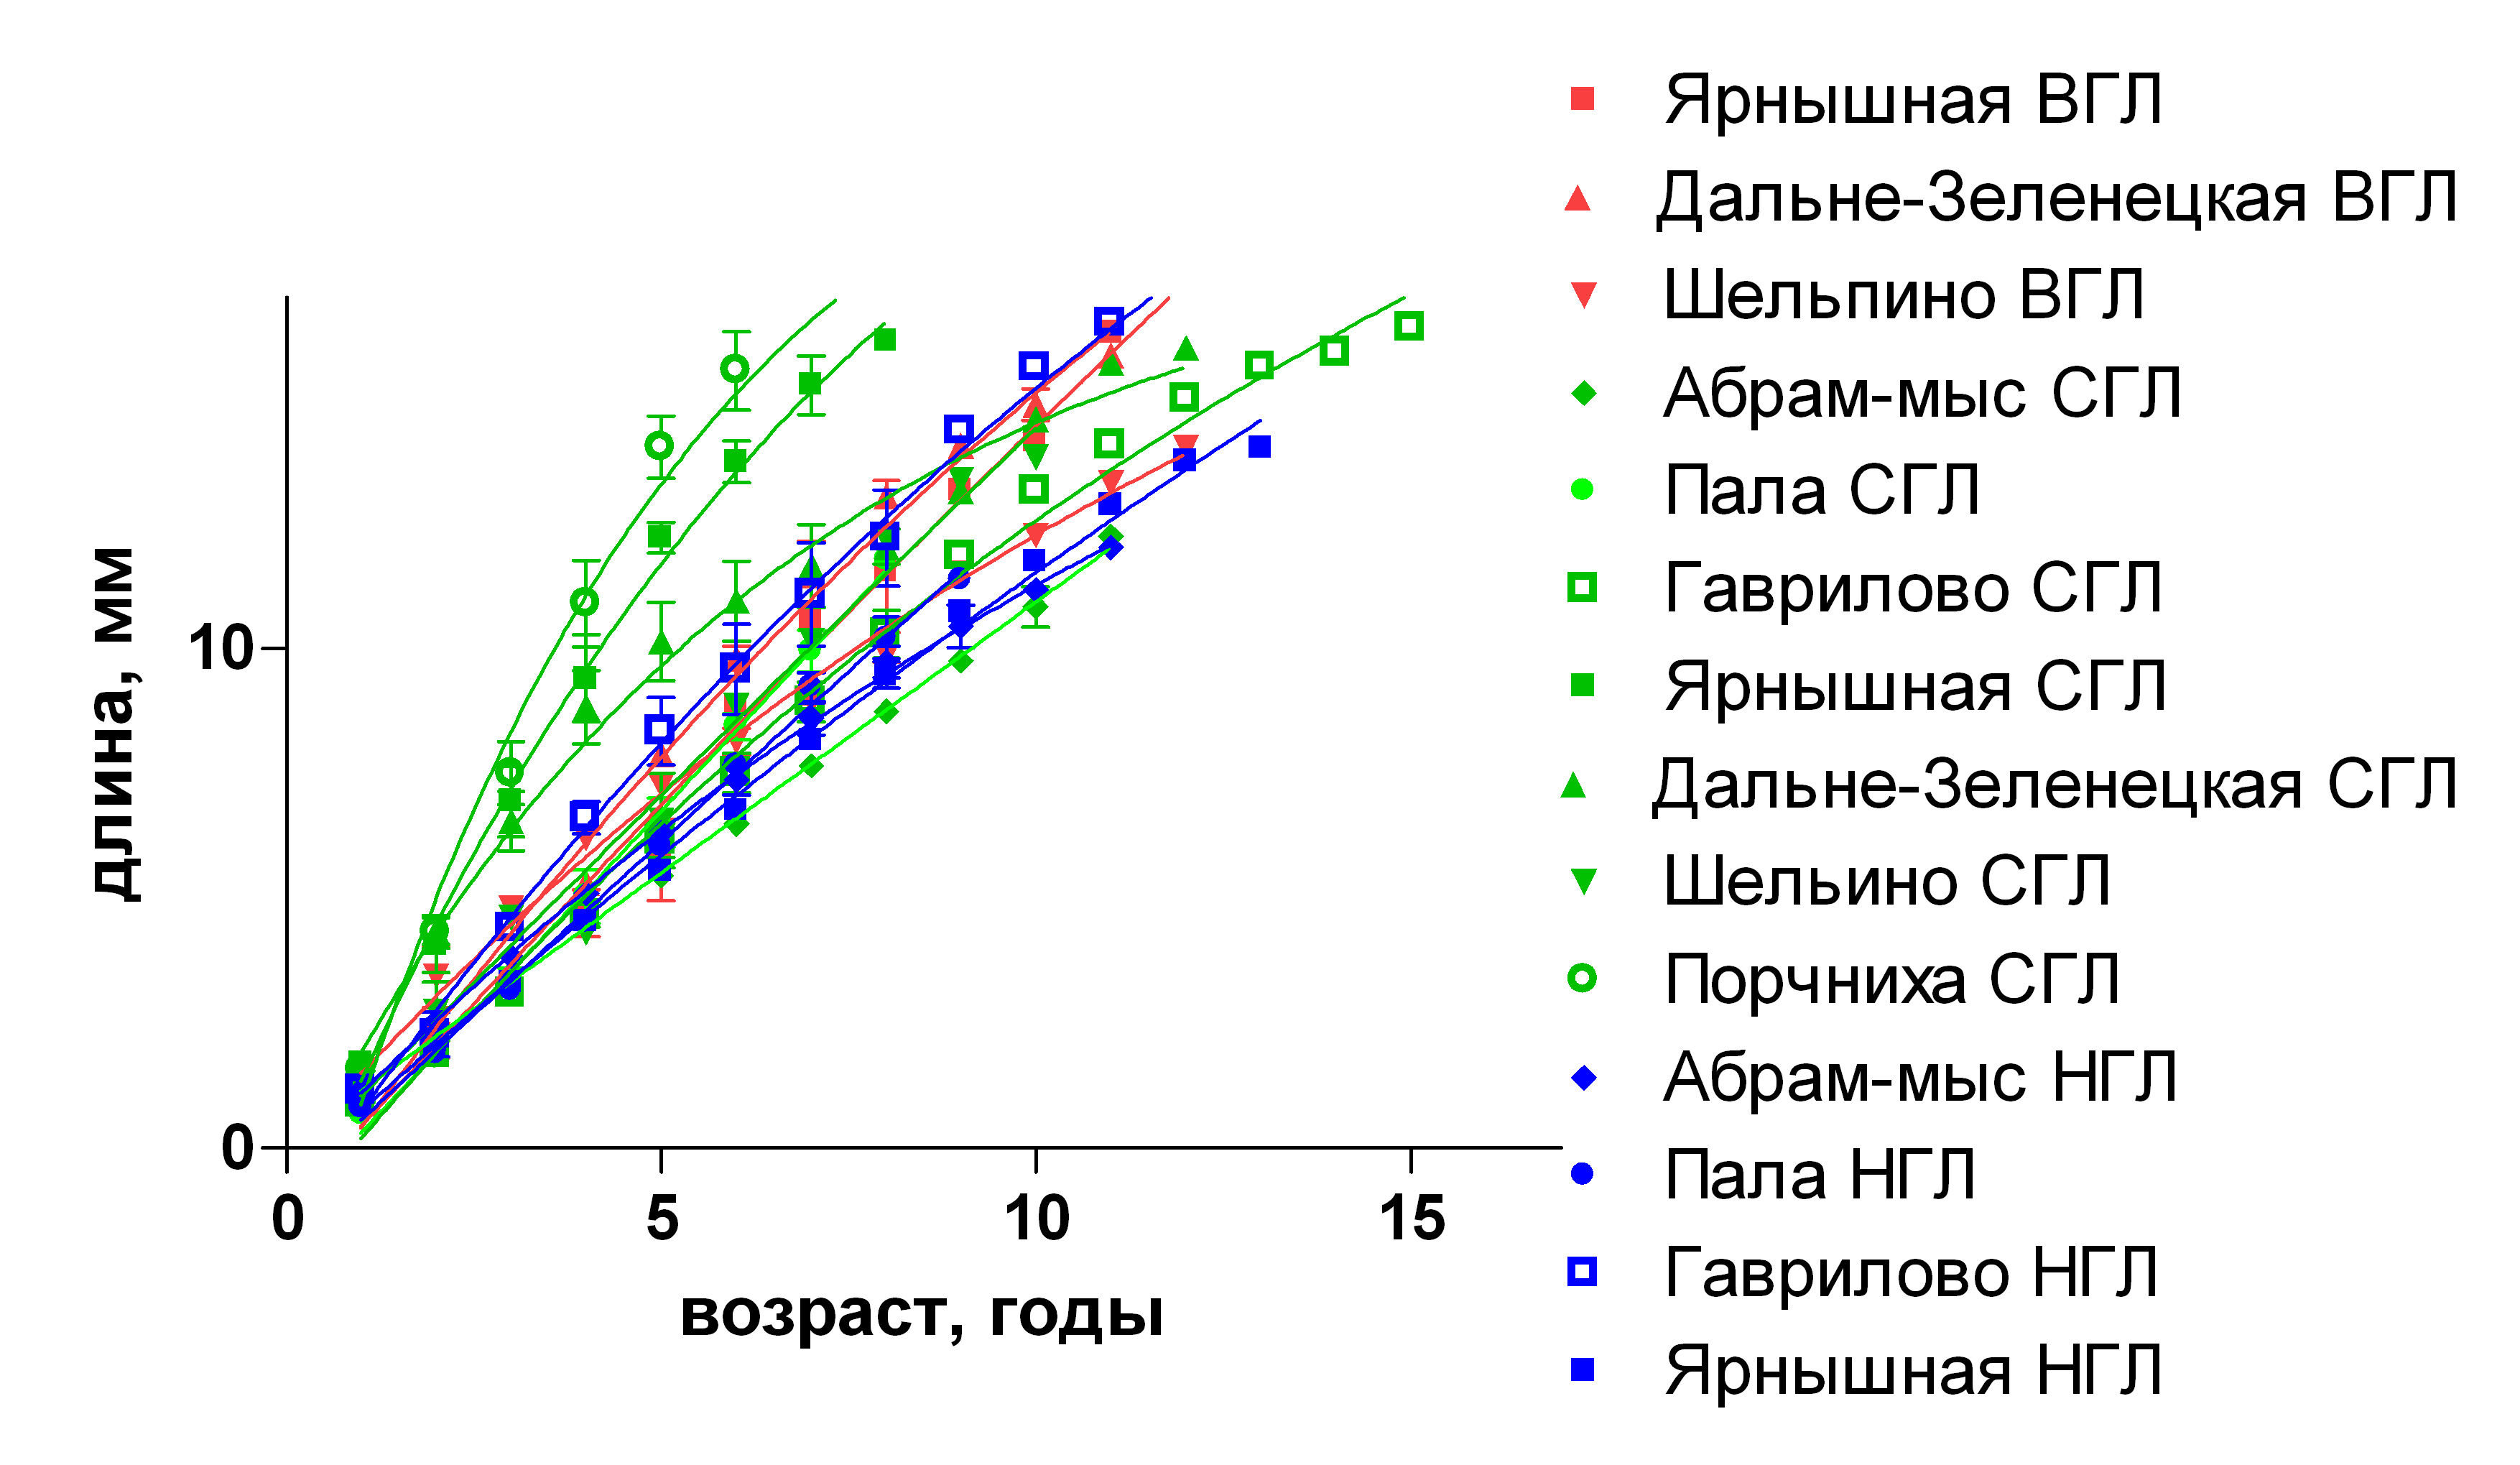
\includegraphics[width=\textwidth]{Rost_gorizonts_all.jpg}\\
	\tiny{Модели линейного роста {\it Macoma balthica} в Баренцевом море}\\
			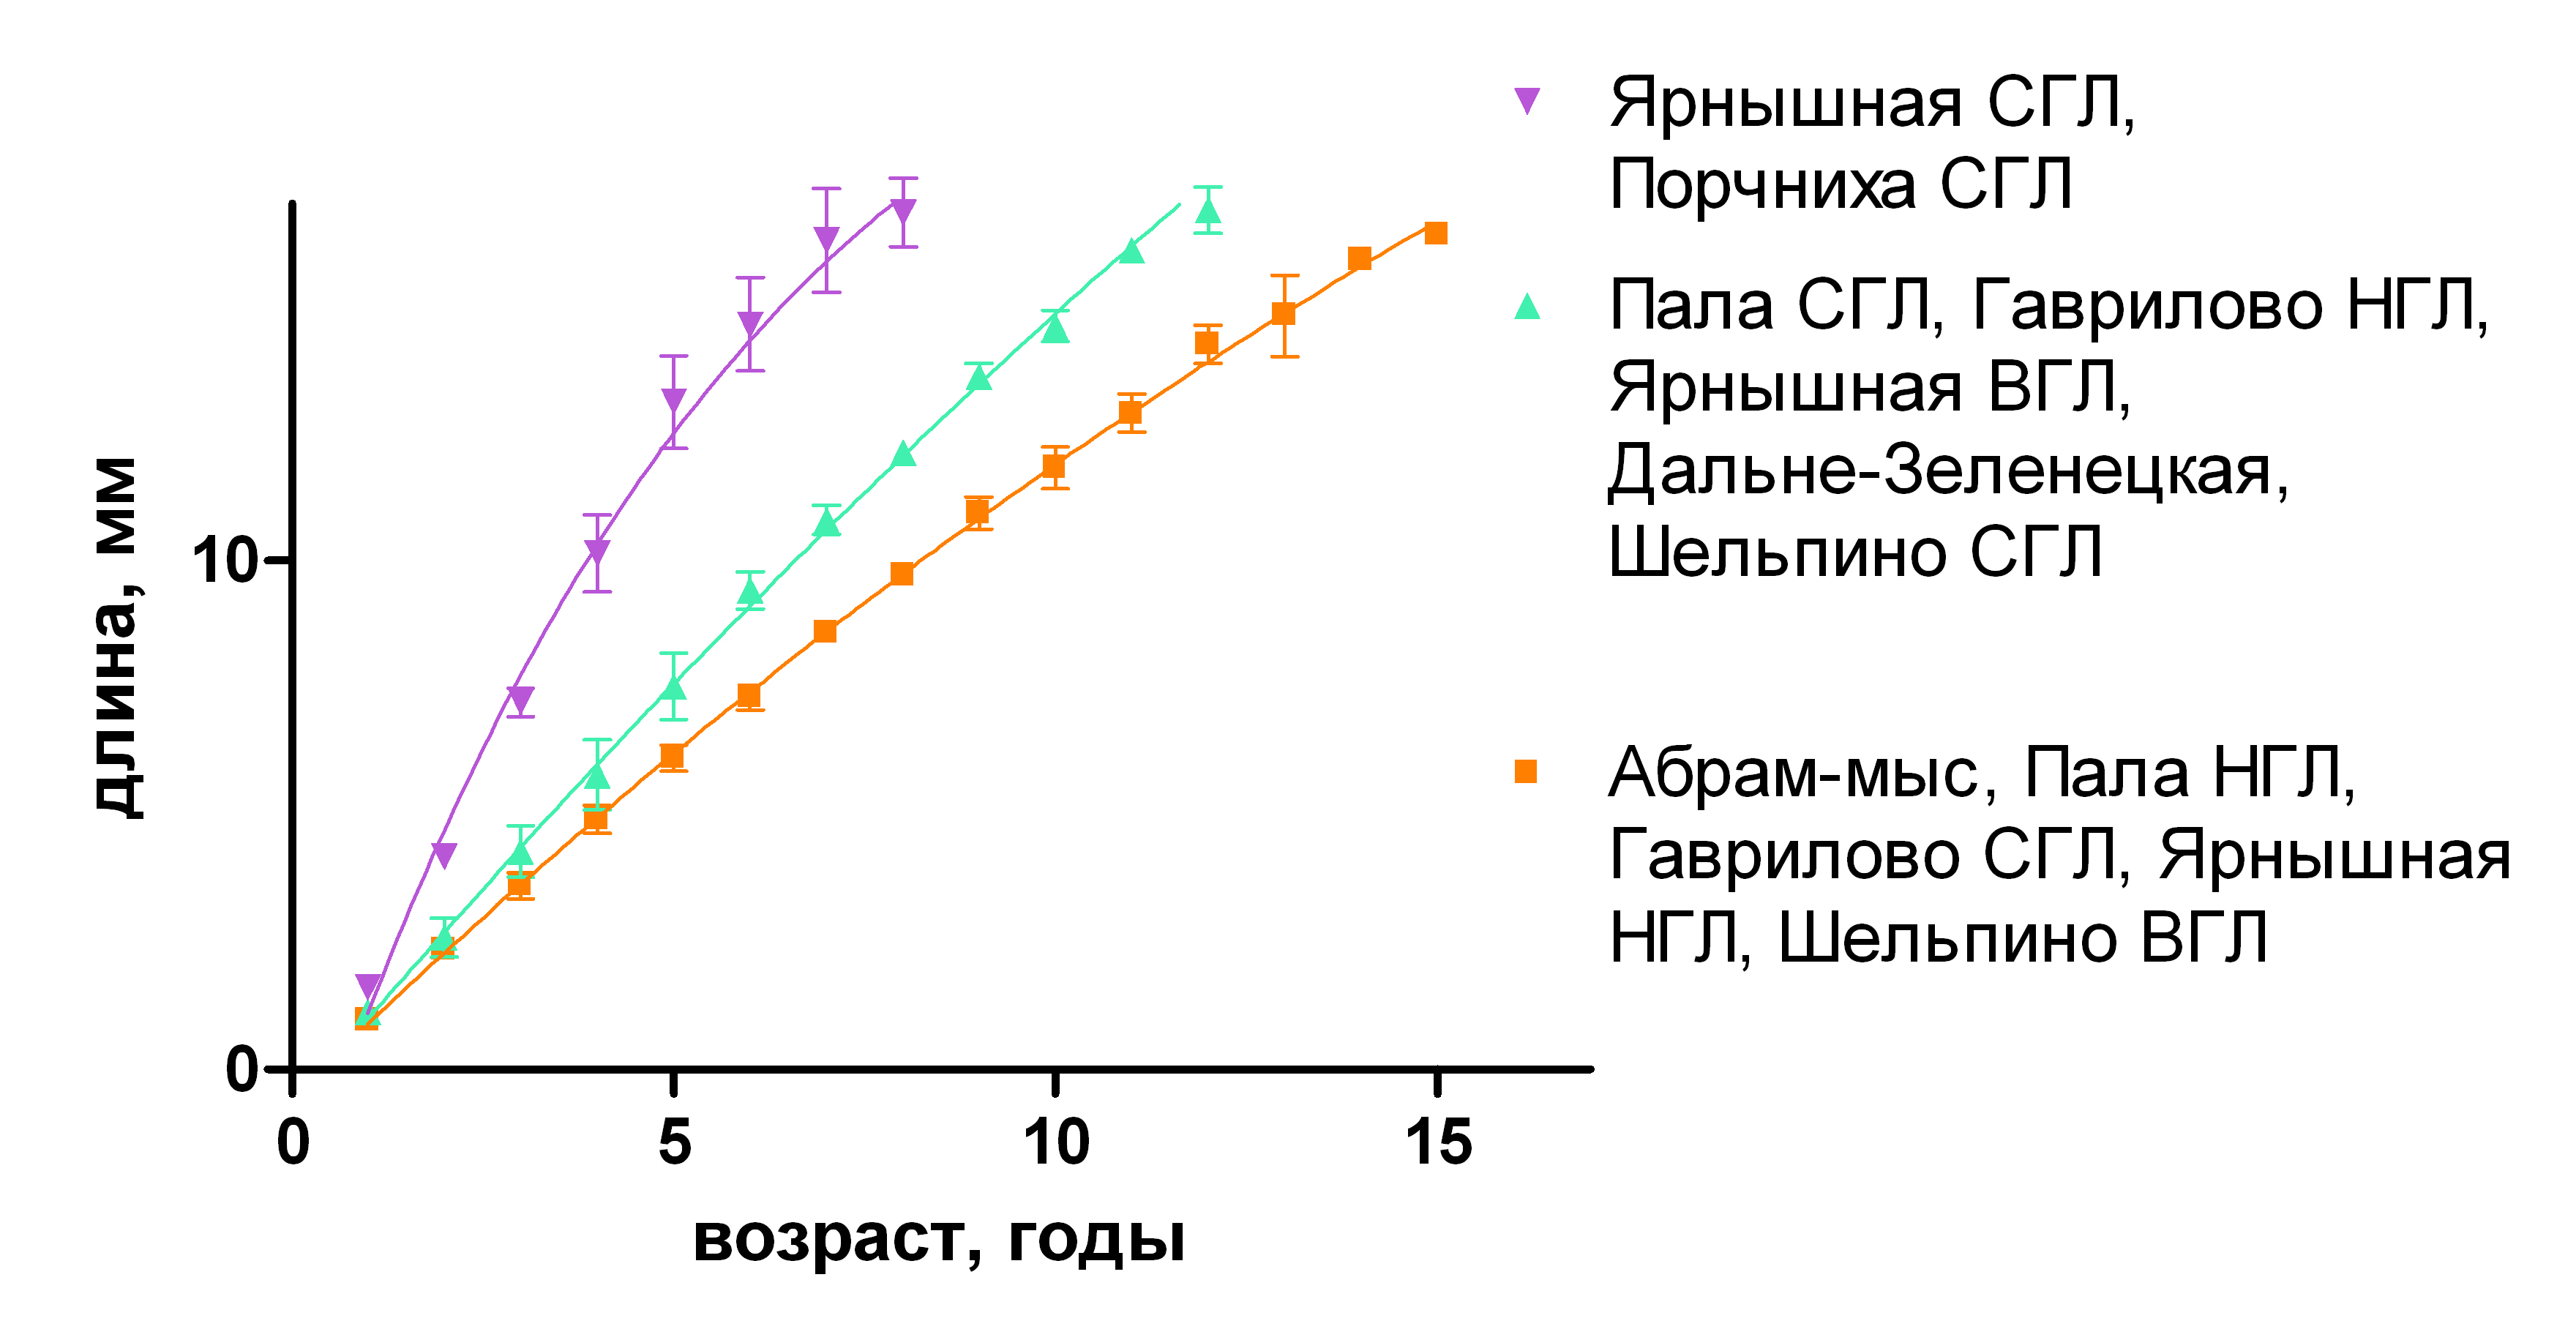
\includegraphics[width=\textwidth]{rost_clusters_all.jpg}
\end{center}
	\end{minipage}
	\begin{minipage}[t]{.3\linewidth}
	\tiny{Классификация кривых роста {\it Macoma balthica} в Баренцевом море}
			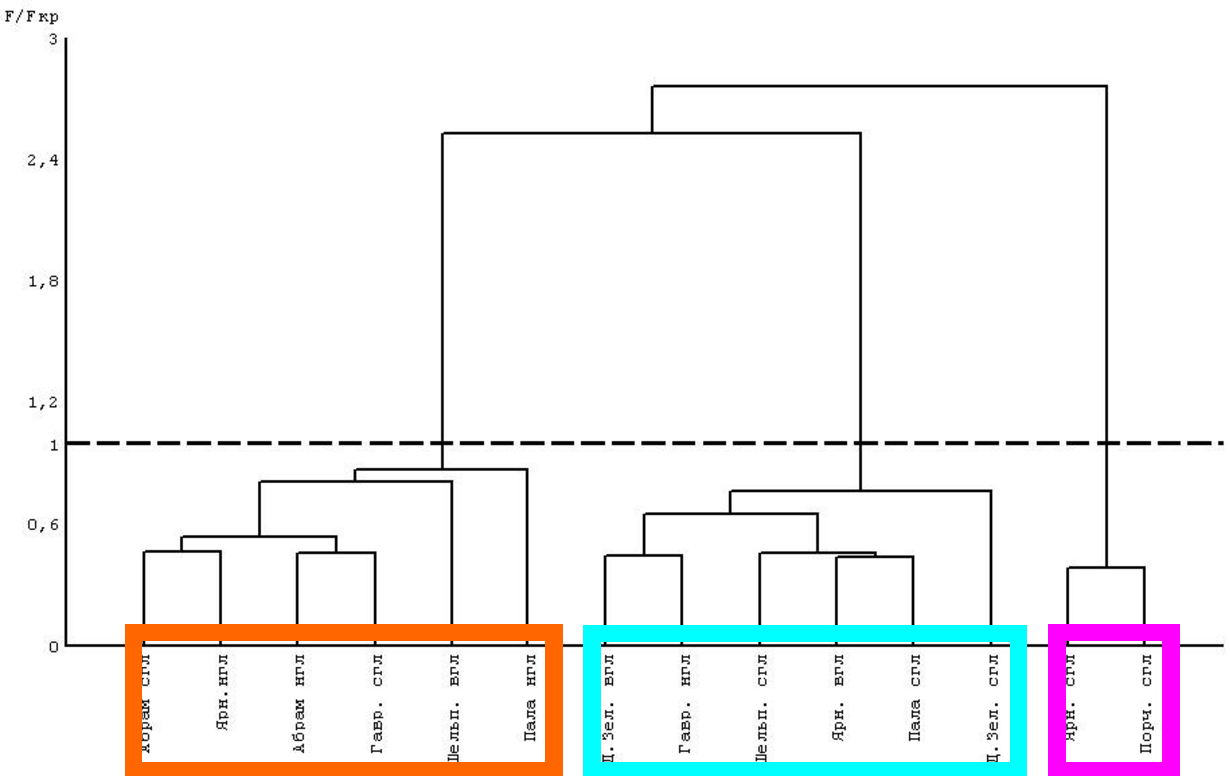
\includegraphics[height=\textwidth, angle=90]{dendrogramma_sravnenie_rosta_linear_all_gorizonts.pdf}
	\end{minipage}
\end{frame}

\begin{frame}{Годовой прирост}
	\begin{minipage}[t]{.45\linewidth}
\begin{center}
	\tiny{Зависимость годового прироста от горизонта литорали}\\
			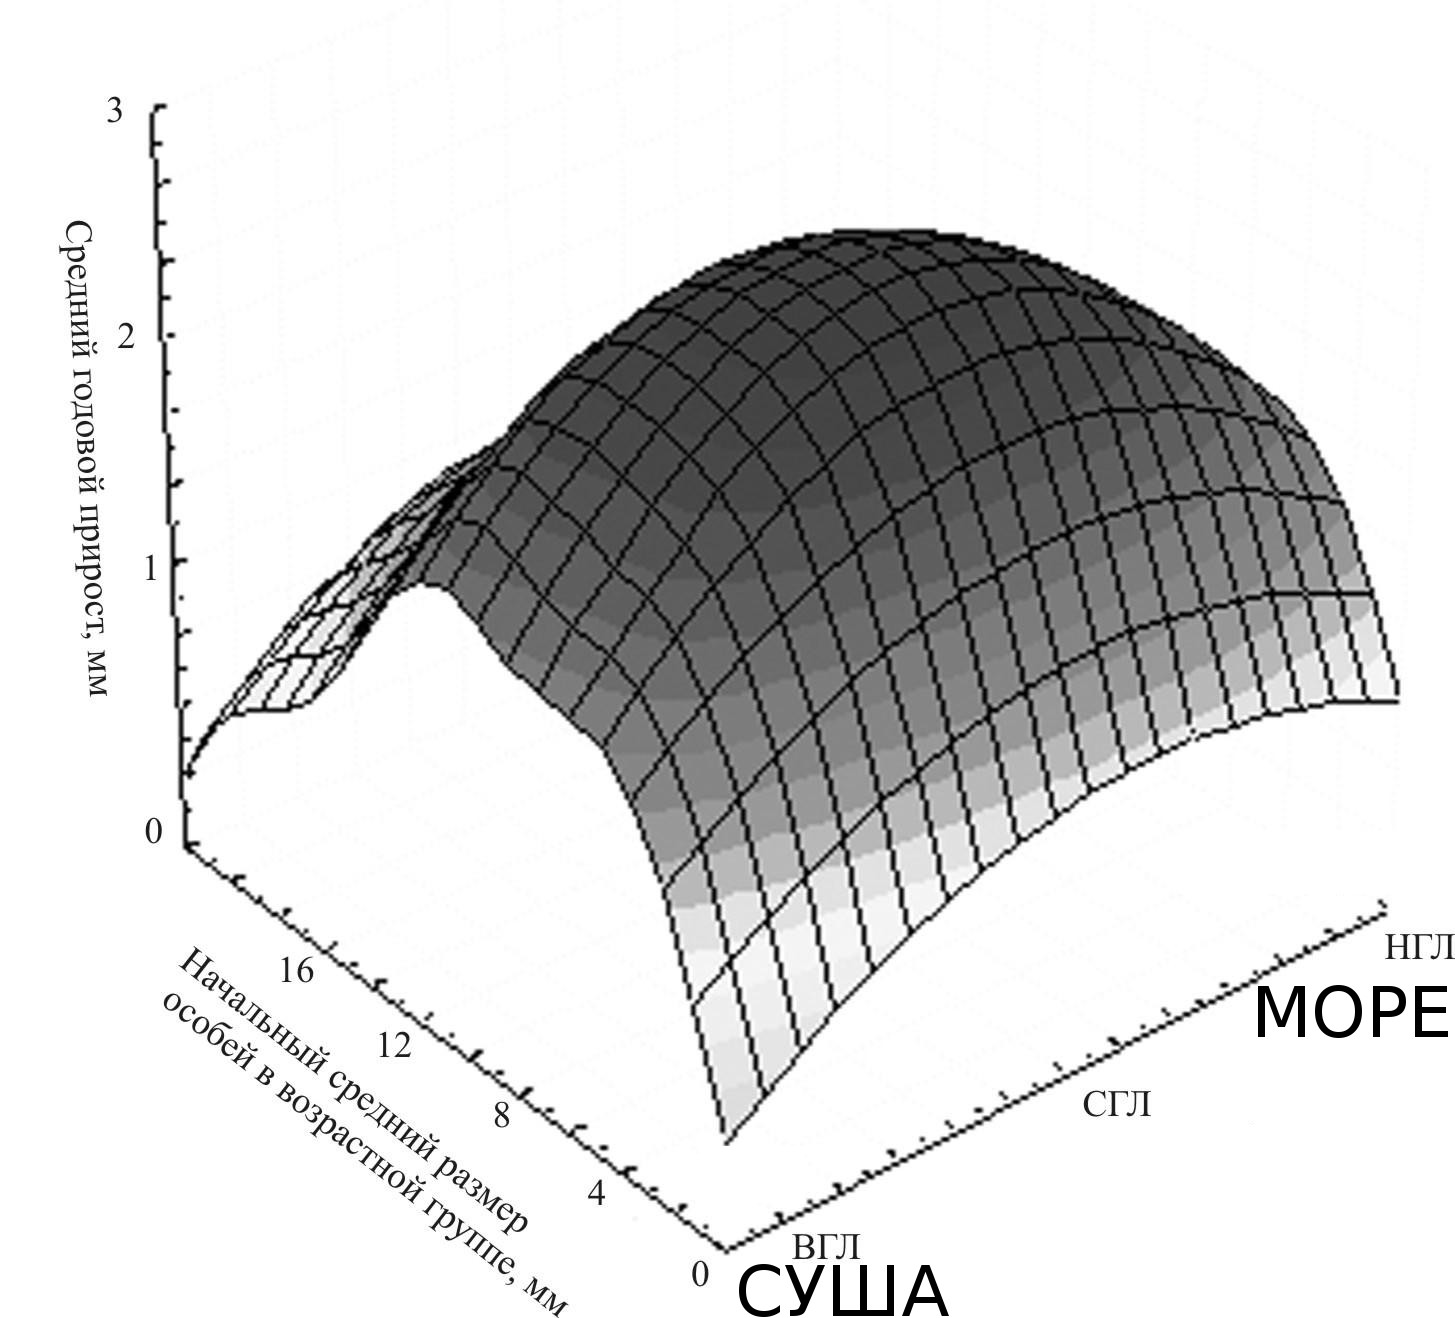
\includegraphics[width=\textwidth]{prirost_otklik_mareography.jpg}\\
\end{center}
	\end{minipage}
	\begin{minipage}[t]{.45\linewidth}
	\tiny{Зависимость годового прироста от географического положения}
			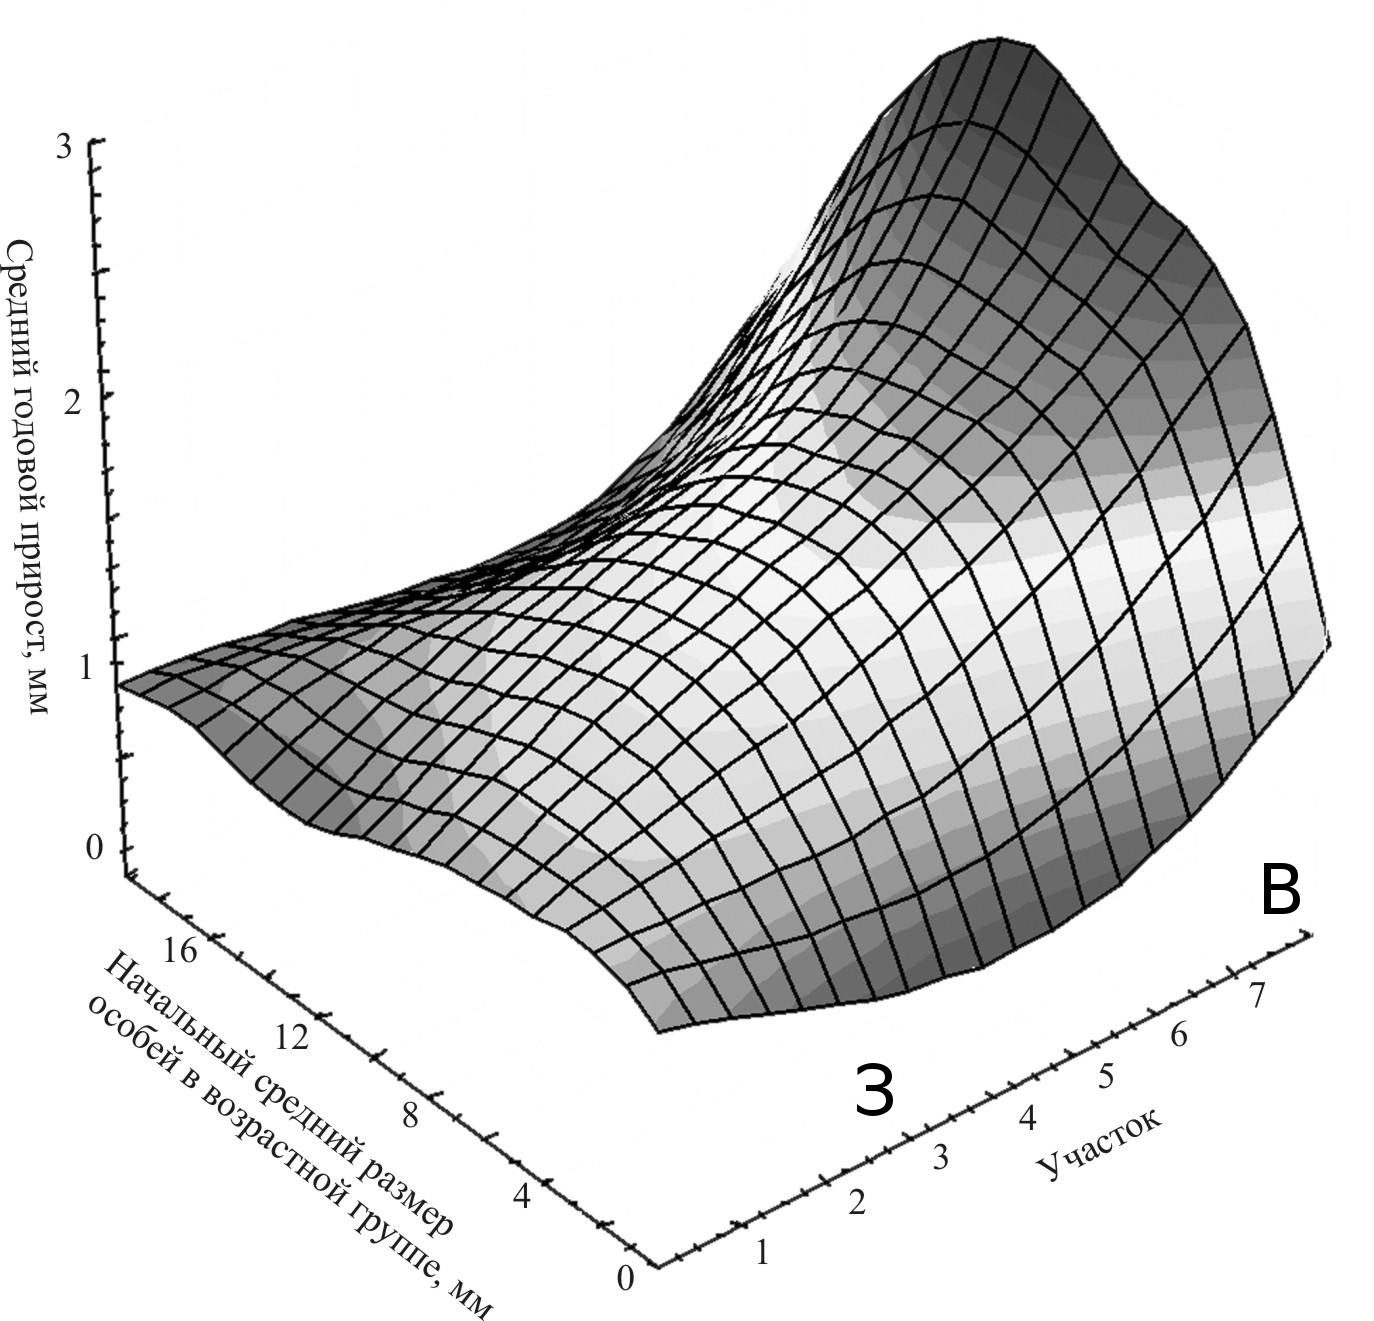
\includegraphics[height=\textwidth]{prirost_otklik_geography.jpg}
	\end{minipage}
\end{frame}

\begin{frame}{Широтное сравнение темпов роста}
Beukema, Meehan (1985): Latitudinal variation in linear growth and other shell characteristics of {\it Macoma balthica}
 \begin{center}
			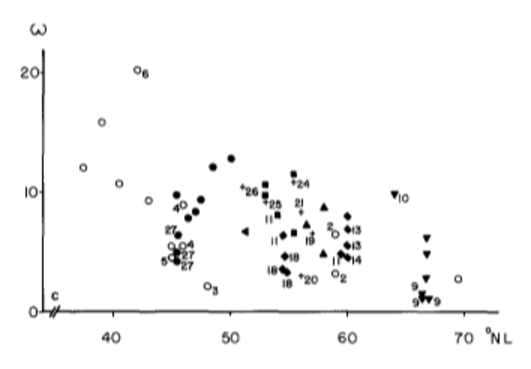
\includegraphics[height=.7\textheight]{from_Bukma_Meehan_1985.pdf}
 \end{center}
\end{frame}

\begin{frame}{Широтное сравнение темпов роста}
 \begin{center}
			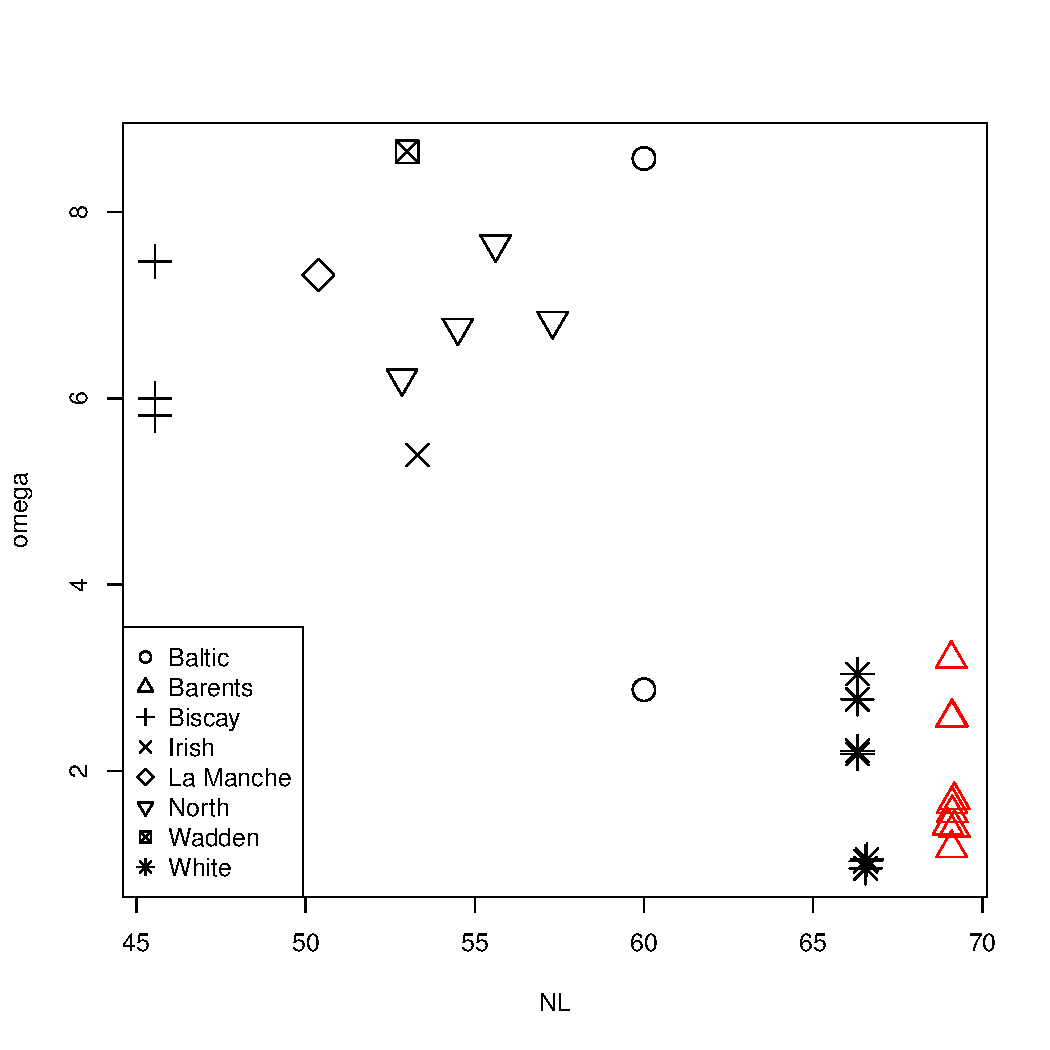
\includegraphics[height=.7\textheight]{long_vs_omega_big.pdf}
 \end{center}
$Spearman\ \rho = -0,59$, $p < 0,001$

\end{frame}

\begin{frame}{Сравнение темпов роста}
	\begin{minipage}[t]{.6\linewidth}
\begin{center}
%	\tiny{Линейный рост {\it Macoma balthica} в Баренцевом море}\\
			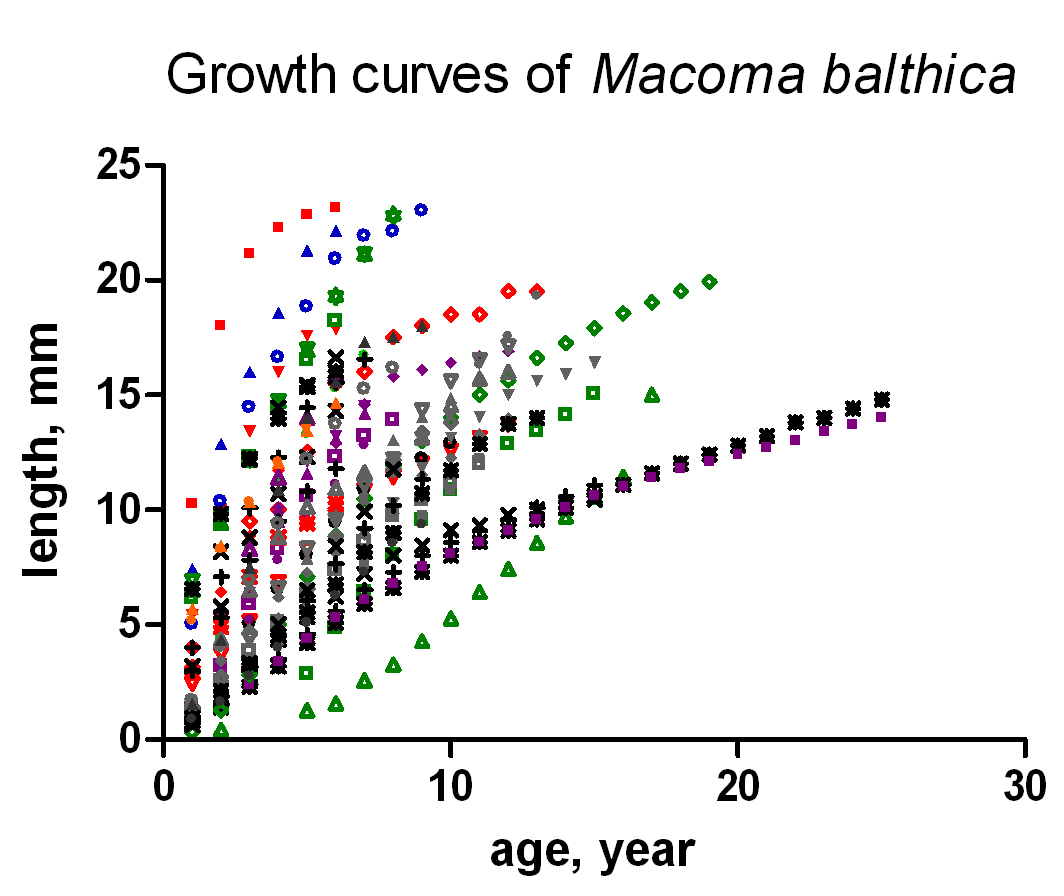
\includegraphics[height=.45\textheight]{curves_Macoma_pict.jpg}\\
%	\tiny{Модели линейного роста {\it Macoma balthica} в Баренцевом море}\\
			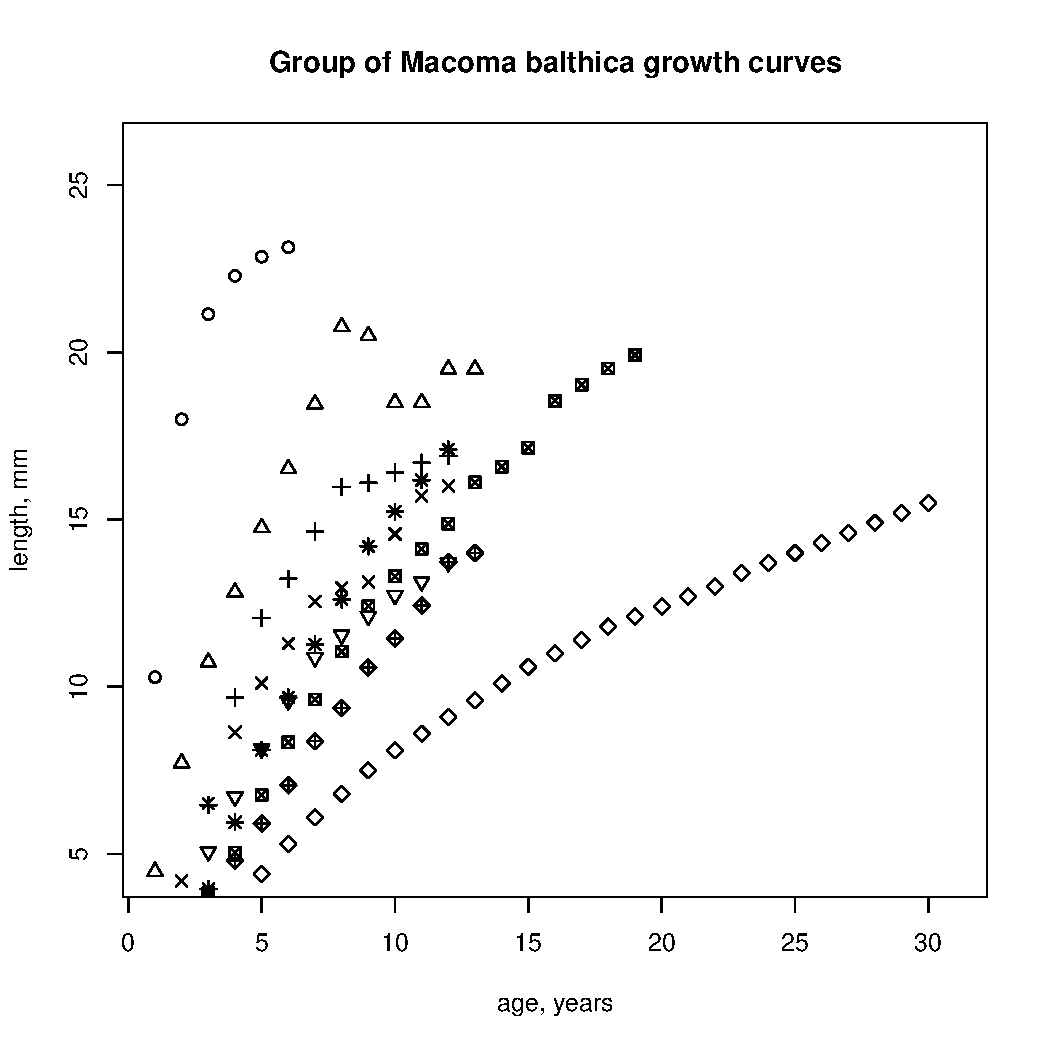
\includegraphics[height=.45\textheight]{clusters_literature.pdf}
\end{center}
	\end{minipage}
	\begin{minipage}[t]{.3\linewidth}
%	\tiny{Классификация кривых роста {\it Macoma balthica} в Баренцевом море}
			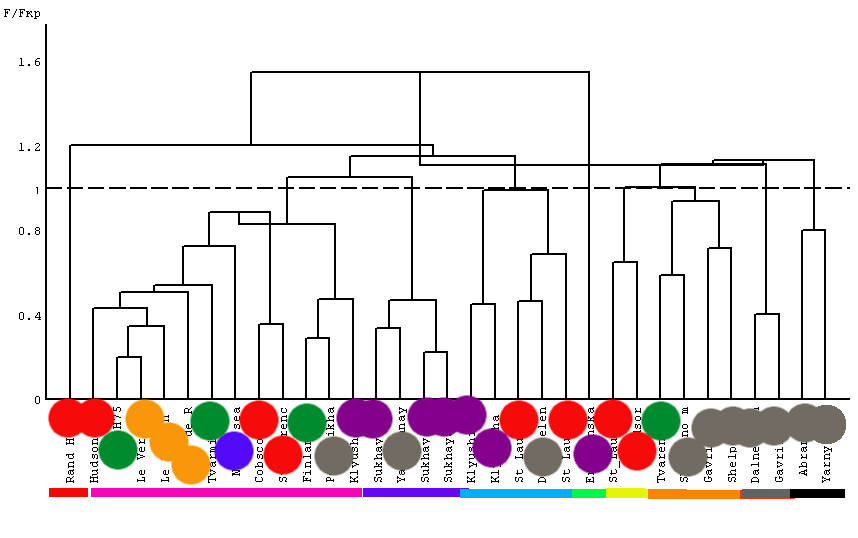
\includegraphics[height=.9\textwidth, angle=90]{dendrogramma_Bertalanfi_obedinenie_col.jpg}
	\end{minipage}
\end{frame}

\begin{frame}{Основные результаты: рост}
	\begin{enumerate}
		\item Макомы в Баренцевом море гетерогенны по скорости роста и выделяется три группы, различающиеся по данному показателю
		\item Максимальный годовой прирост отмечен у особей среднего размера (возраста) --- $6 - 9$~мм
		\item Максимальный годовой прирост в Баренцевом море наблюдается в среднем горизонте литорали
		\item В пределах Восточного Мурмана средний годовой прирост увеличивается в более восточных районах по сравнению с западными
		\item Полученные для Баренцева моря данные о росте маком в целом соответствуют существующим представлениям о широтном изменении темпов роста, однако вариабельность данного параметра очень высока и подвержена влиянию локальных факторов.
	\end{enumerate}
\end{frame}

		\section[Динамика обилия]{Динамика обилия {\it Macoma balthica}}
\begin{frame}{Материал и методы: динамика}
\begin{itemize}
	\item Белое море: 6 участков в районе Кандалакши
	\item Баренцево море: 1 участок в губе Дальнезеленецкая
	\item Длина рядом от 6 до 21 года
	\item Пробоотбор ежегодный, повторность 3 -- 25 проб
	\item рамка 1/30 или 1/10~м$^2$, сито 0,5 или 1~мм.
	\item Плотностнозависимые процессы: метод частных корреляций PRCF --- partial rate correlation function (Berryman, Turchin, 2001). \\
{\footnotesize Logarithmic per-capita rate of change $Rt =\ln(N_{t}/N_{t - 1})$. \\ Модель: $Rt = L_{t} - L_{t - 1} = a_{0} + a_{1}L_{t - 1} + a_{2}L_{t - 2} + \cdots + a_{d}L_{t - d} + \epsilon_{1}$}
	\item Наличие трендов и синхронность динамики: корреляции Мантеля
\end{itemize}
\end{frame}

\begin{frame}{Динамика обилия}
	\begin{minipage}[t]{.45\linewidth}
\begin{center}
			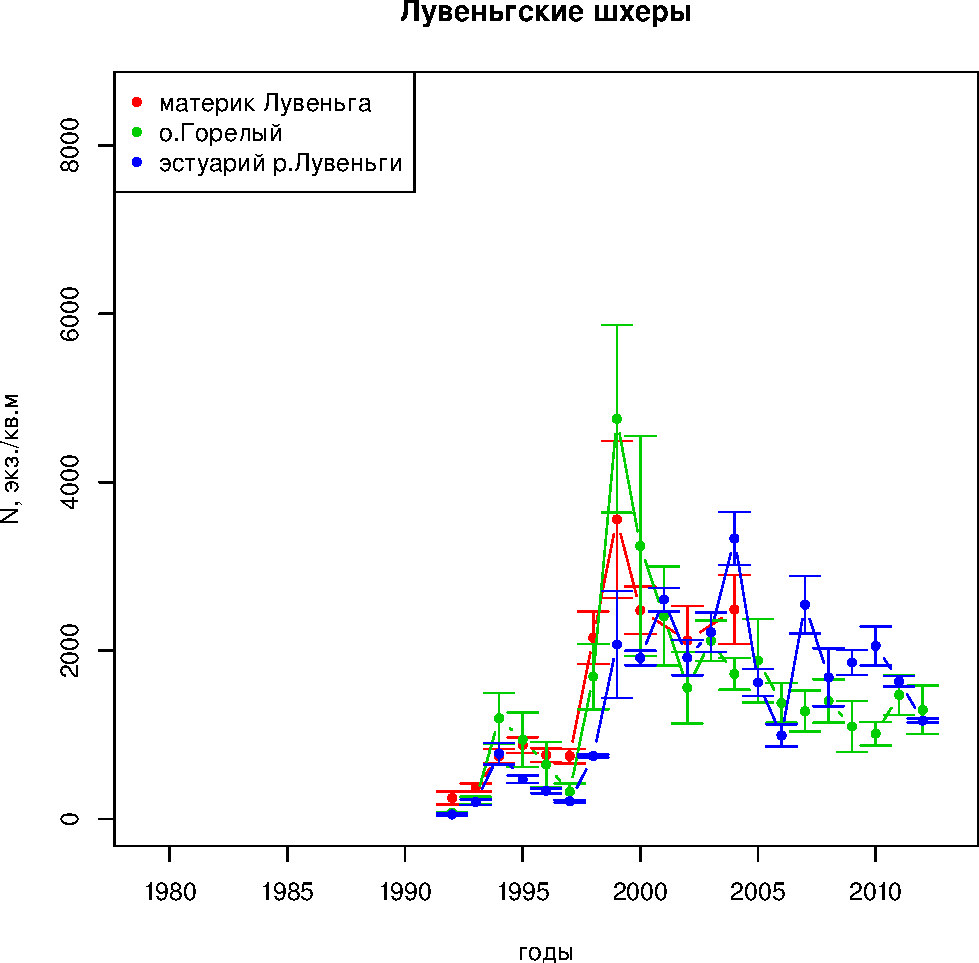
\includegraphics[height=.45\textheight]{N2_dynamic_Luvenga_all.pdf}\\
			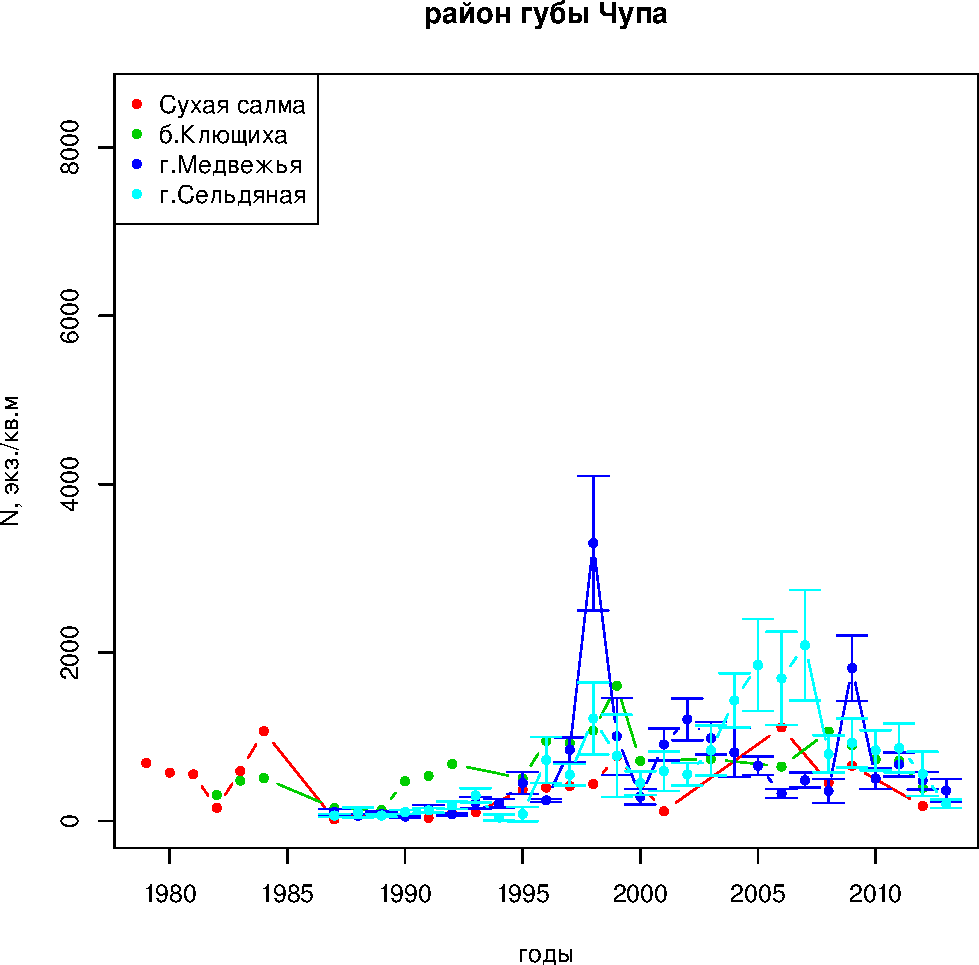
\includegraphics[height=.45\textheight]{N2_dynamic_Chupa_all.pdf}
\end{center}
	\end{minipage}
	\begin{minipage}[t]{.45\linewidth}
			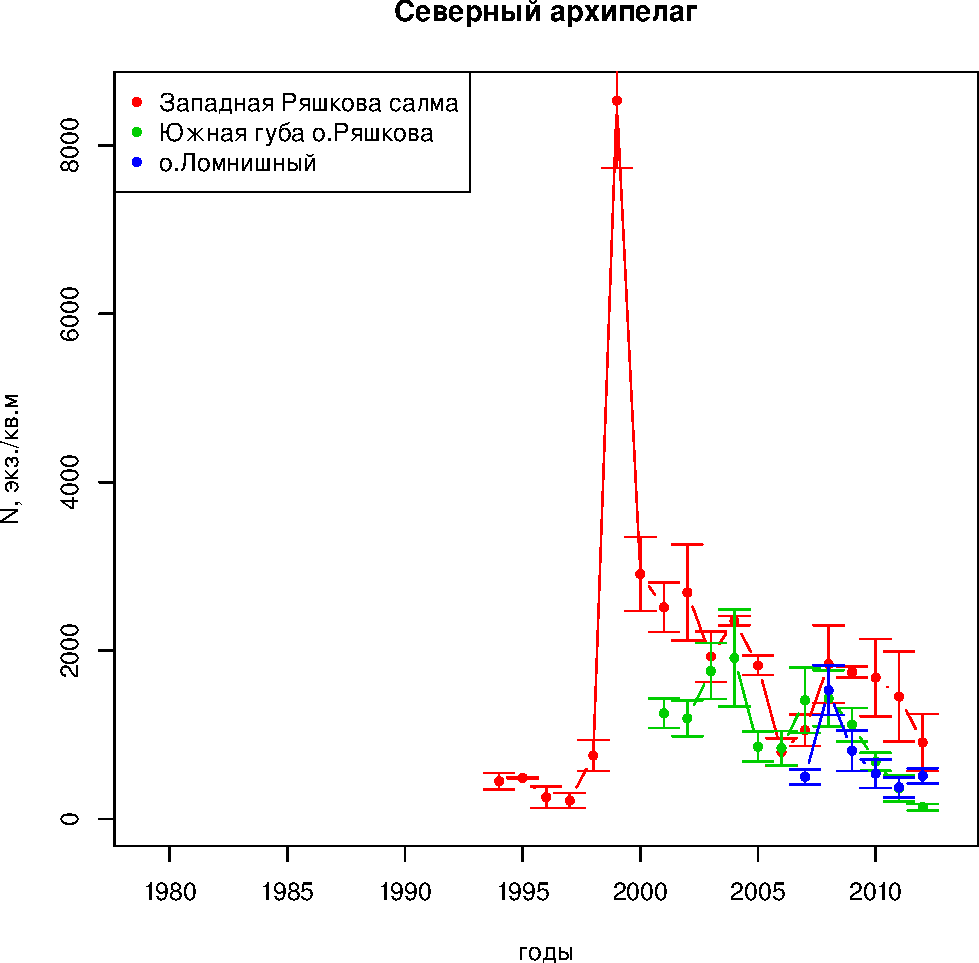
\includegraphics[height=.45\textheight]{N2_dynamic_North_all.pdf}
	\end{minipage}
\end{frame}

\begin{frame}{Синхронность динамики}
 \begin{center}
		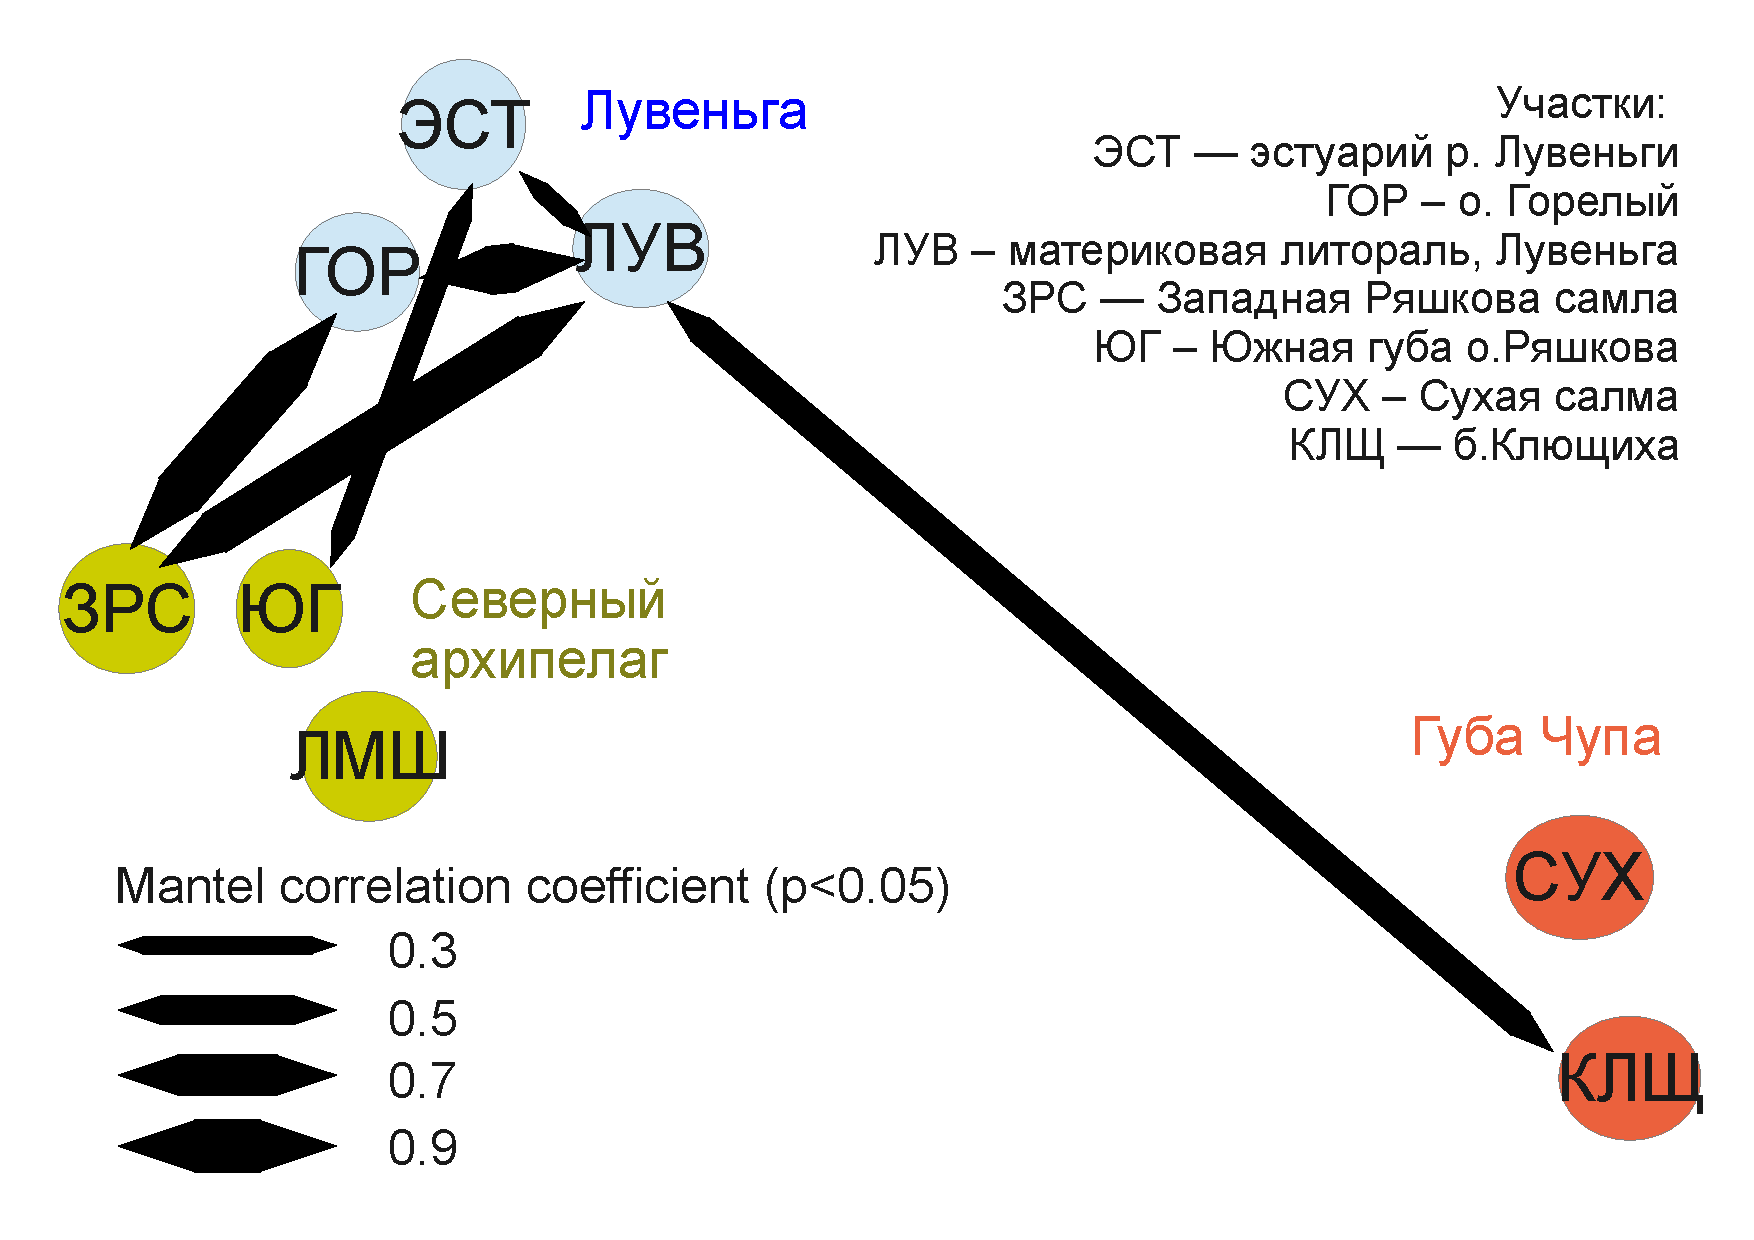
\includegraphics[width=.8\textwidth]{Mantel_shema.pdf}
 \end{center}
Корреляция с расстоянием между участками: $Mantel\ r = - 0,1$, $p = 0,64$
\end{frame}

\begin{frame}{Плотностнозависимые процессы}
 \begin{center}
		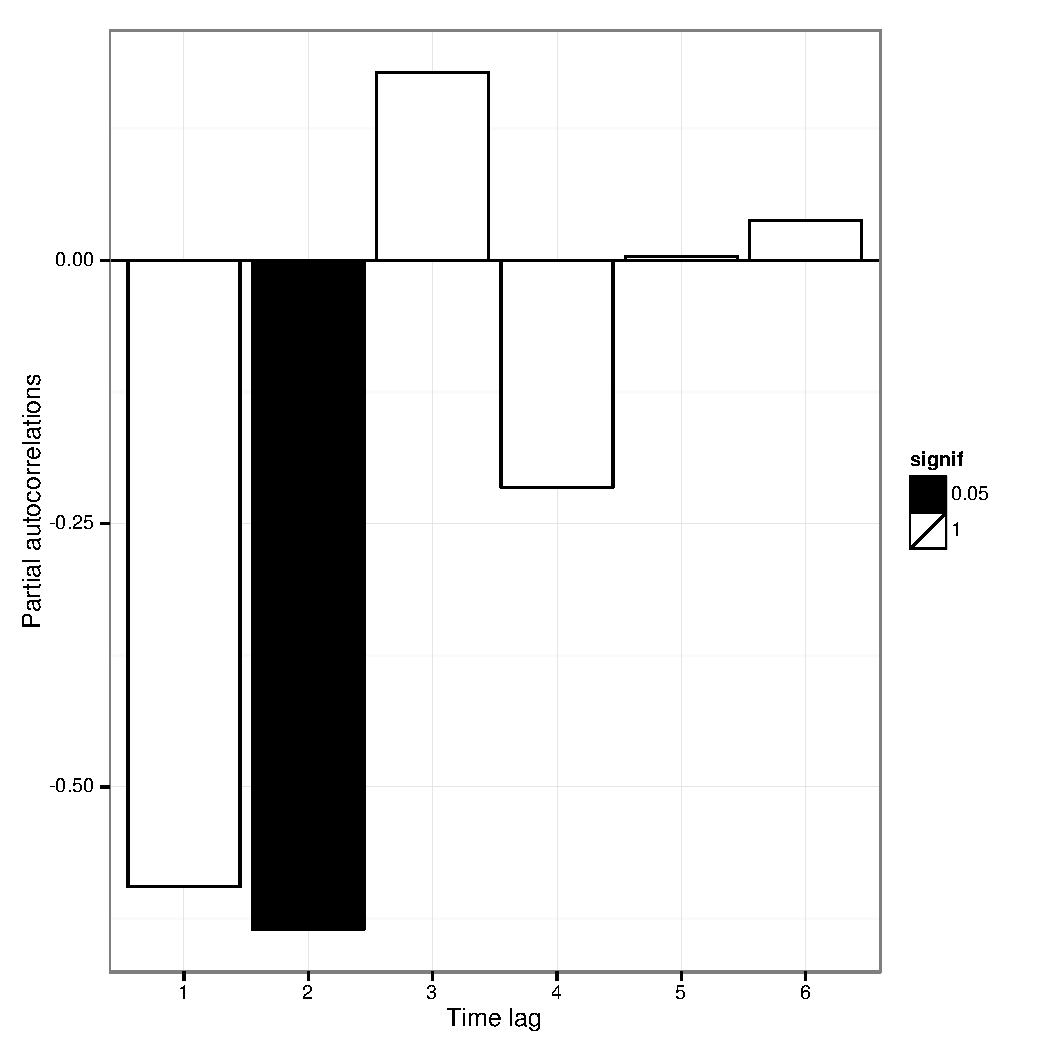
\includegraphics[width=.8\textwidth]{perm_PRCF_YuG_detrend.pdf}
 \end{center}
\end{frame}




\begin{frame}{Основные результаты: динамика}
	\begin{enumerate}
		\item Изменения плотности поселений маком связаны в первую очередь с частотой пополнения поселений молодью
		\item Во всех исследованных поселениях в 1998-1999 году было отмечено достоверное увеличение численности маком 
		\item Обнаружены элементы синхронности в динамике поселений, расположенных на расстоянии от 1 до 100 км
		\item Расстояние между участками не коррелирует со степенью синхронности динамики поселений
	\end{enumerate}
\end{frame}

		\section{Пополнение поселений {\it Macoma balthica}}
\begin{frame}{Материал и методы: пополнение}
\begin{itemize}
	\item Белое море: 6 участков в районе Кандалакши
	\item Длина рядом от 6 до 21 года
	\item Пробоотбор ежегодный, повторность 3 -- 25 проб
	\item рамка 1/30 или 1/10~м$^2$, сито 0,5 или 1~мм.
	\item По данным 2013 года --- определение длины раковины годовалых особей
	\item По данным о размерах моллюсков вычисление численности годовалых маком
	\item Губа Чупа, 2006 год: однократная съемка в сентябре на обилие спата
\end{itemize}
\end{frame}

%\begin{frame}{Размер годовалых особей}
% \begin{center}
%
% \end{center}
%\end{frame}

\begin{frame}{Динамика пополнения поселений}
	\begin{minipage}[t]{.45\linewidth}
\begin{center}
			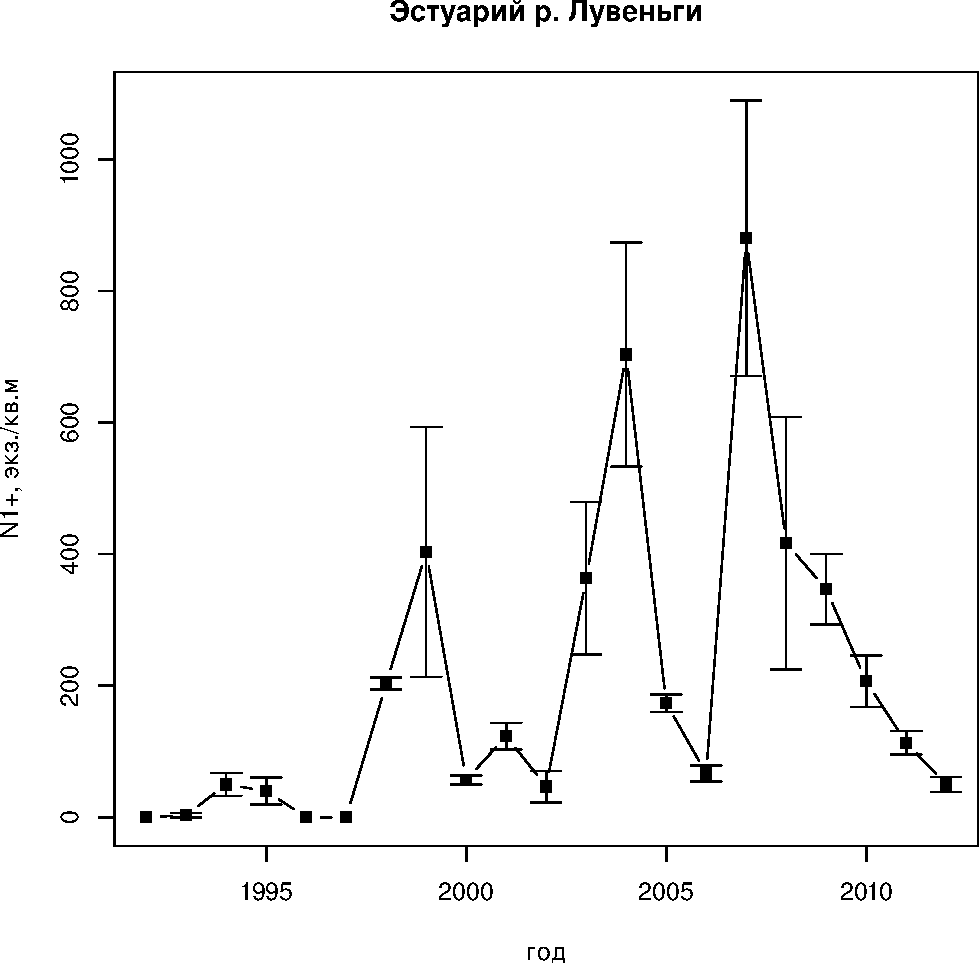
\includegraphics[height=.45\textheight]{Estuary_N_oneyear.pdf}\\
			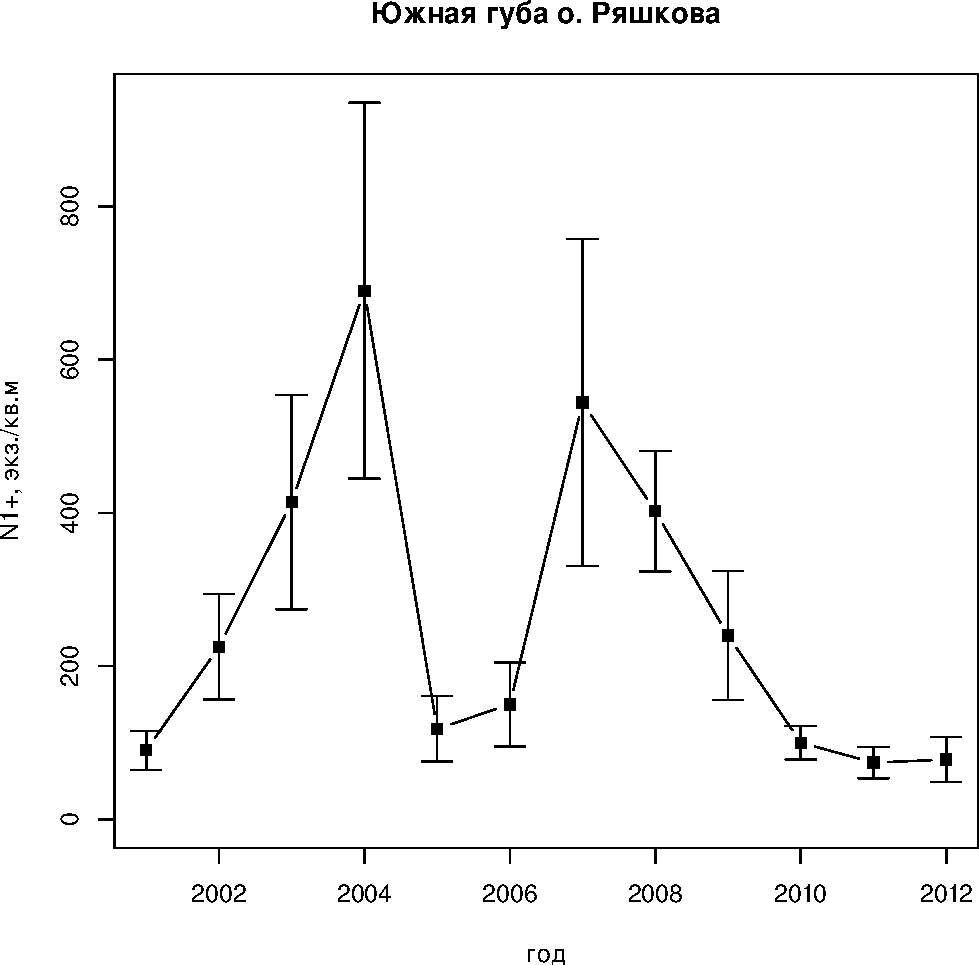
\includegraphics[height=.45\textheight]{YuG_N_oneyear.pdf}
\end{center}
	\end{minipage}
	\begin{minipage}[t]{.45\linewidth}
			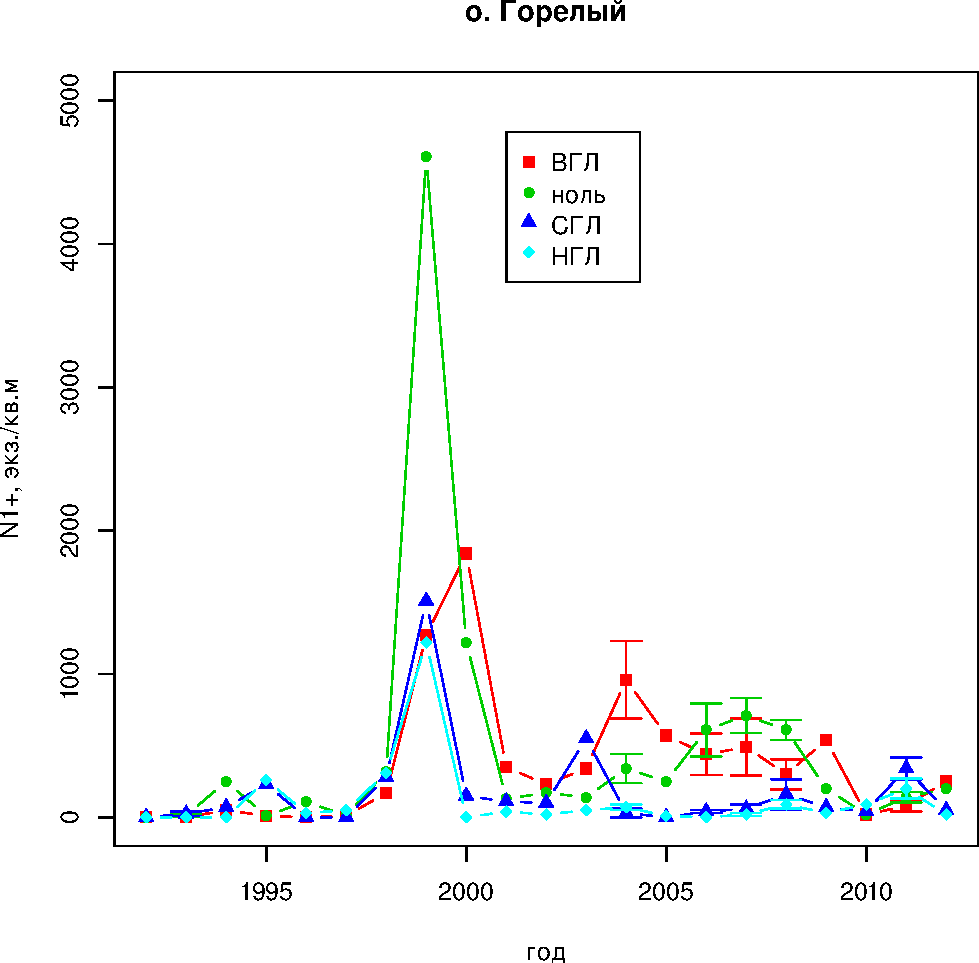
\includegraphics[height=.45\textheight]{Goreliy_N_oneyear.pdf}\\
			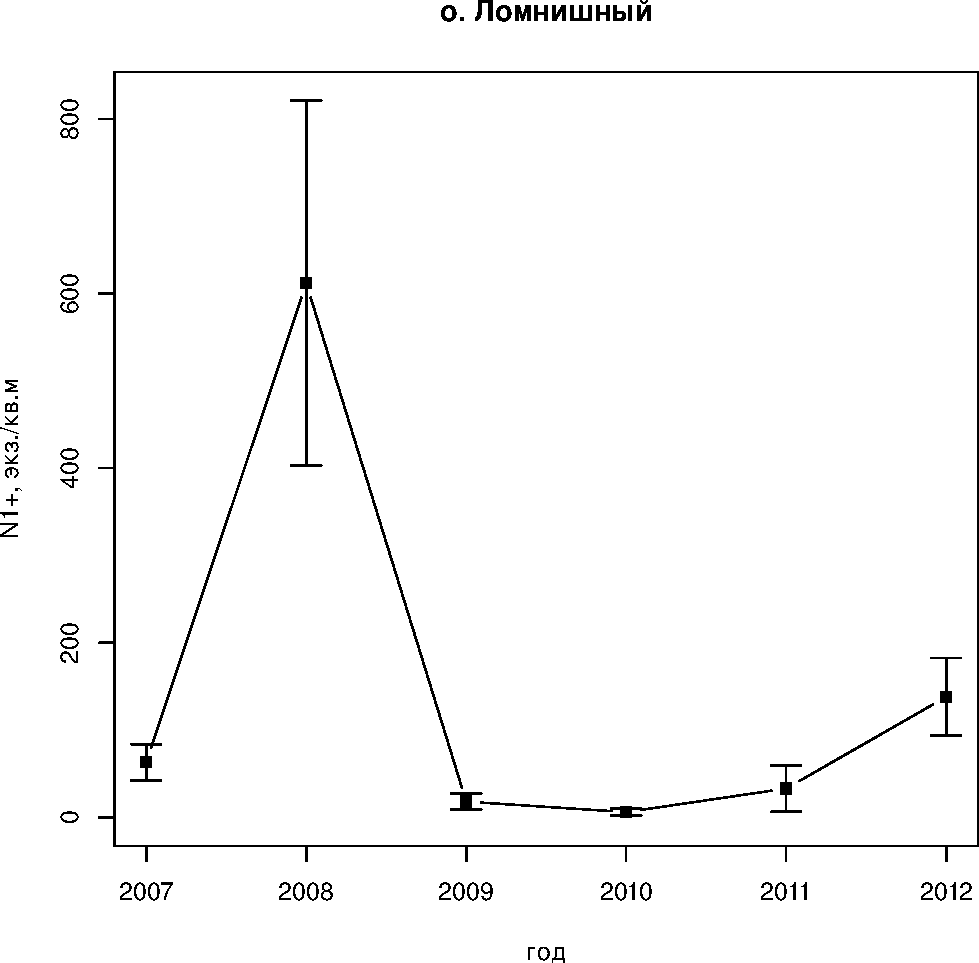
\includegraphics[height=.45\textheight]{Lomnishniy_N_oneyear.pdf}
	\end{minipage}
\end{frame}


\begin{frame}{Влияние числа половозрелых особей на пополнение поселения молодью}
 \begin{center}
	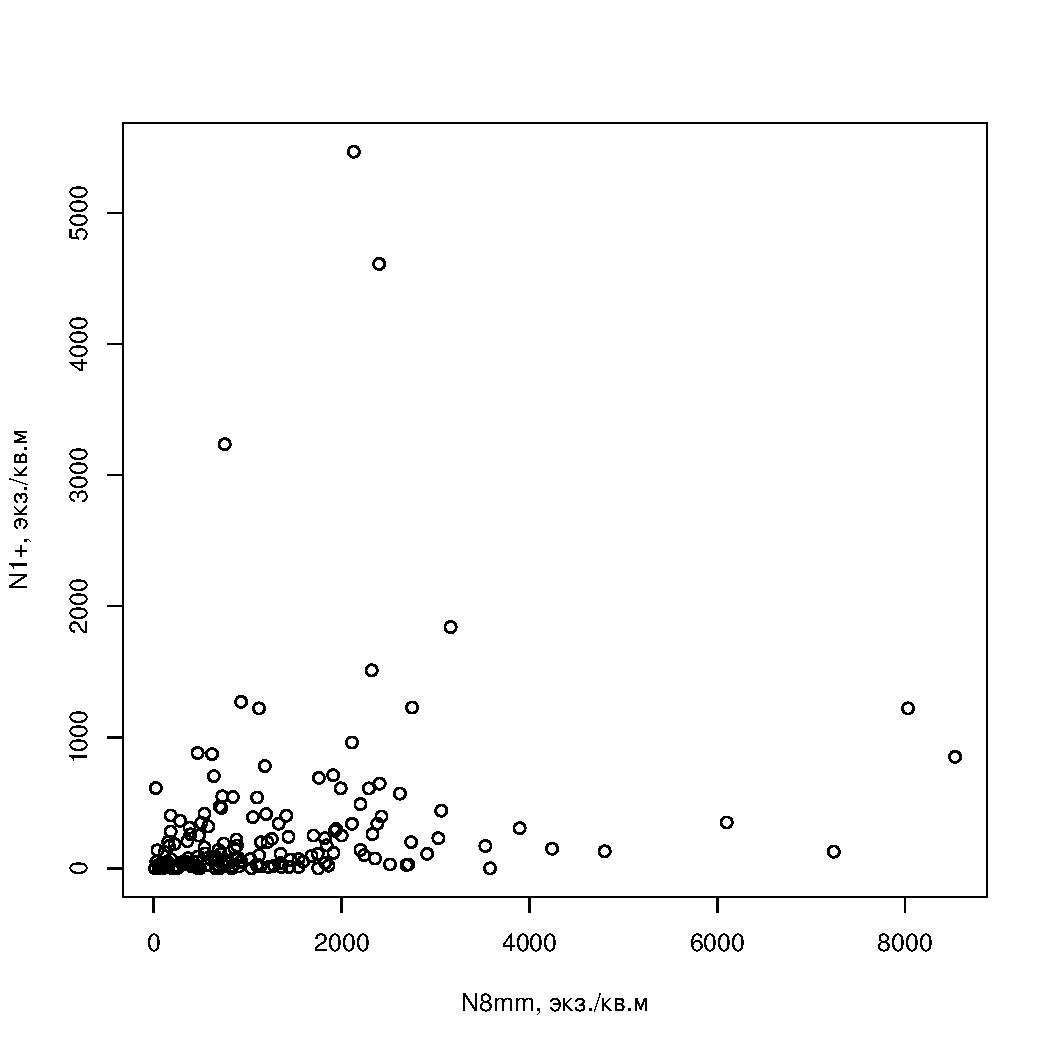
\includegraphics[height=.6\textheight]{N8mm_vs_N1y_1.pdf}
 \end{center}
$Spearman\ \rho = 0,39$, $p < 0,0001$

\end{frame}

\begin{frame}{Основные результаты: пополнение}
	\begin{enumerate}
	\begin{small}
		\item Численность спата может варьировать на порядок в пределах незначительной акватории (4000 -- 10000~экз./м$^2$)
		\item Размерная структура спата в конце лета --- мономодальная, преобладающий размер варьирует от 0,5 до 0,75~мм. 
		\item К концу августа вновь осевшие особи достигают размера 0,3-1,45~мм
		\item Обилие годовалых особей варьирует от 0 до 5500~экз./м$^2$
		\item Динамика годовалых особей позволяет говорить о неежегодном пополнении поселений в Белом море
		\item Флуктуации общего обилия маком во многом связаны с динамикой обилия годовалых особей
		\item Показана слабая положительная корреляция между численностью годовалых особей и численностью половозрелых особей в год оседания
		\item Показана достоверная отрицательная корреляция между численностью взрослых маком и спатом
	\end{small}
	\end{enumerate}
\end{frame}

\begin{small}
		\section{Выводы}
\begin{frame}{Выводы}
	\begin{enumerate}
		\item Для Белого моря типичны поселения {\it Macoma balthica} с численностью  700 -- 800~экз./м$^2$ (при варьировании от 10 до 8500~экз./м$^2$). Варьирование обилия связано в первую очередь с численностью годовалых особей.
		\item Для литорали восточной части Мурманского побережья баренцева моря типичны поселения {\it Macoma balthica} с численностью  менее 100~экз./м$^2$ (при варьировании от 30 до 3350~экз./м$^2$).
		\item Отдельные районы Кандалакшского залива Белого моря не различаются по средней численности особей {\it Macoma balthica}.
		\item Численность особей {\it Macoma balthica} в Баренцевом море на Восточном Мурмане ниже, чем на Западном и в Кольском заливе.
		\item Среднее обилие {\it Macoma balthica} в поселениях Белого моря и Кольского залива Баренцева моря выше, чем в других частях ареала. 
	\end{enumerate}
\end{frame}

\begin{frame}{Выводы}
	\begin{enumerate}
\addtocounter{enumi}{5}
		\item Макомы в Баренцевом море гетерогенны по скорости роста: Максимальный годовой прирост отмечен у особей среднего размера (возраста) --- $6 - 9$~мм в среднем горизонте литорали.
		\item В пределах Восточного Мурмана средний годовой прирост особей {\it Macoma balthica} увеличивается в более восточных районах по сравнению с западными.
		\item Численность спата {\it Macoma balthica} в Белом море может варьировать на порядок в пределах незначительной акватории (4000 -- 10000~экз./м$^2$).
		\item Динамика численности годовалых особей {\it Macoma balthica} позволяет говорить о неежегодном успехе пополнения поселений в Белом море.
	\end{enumerate}
\end{frame}
		
\begin{frame}{Выводы}
	\begin{enumerate}
\addtocounter{enumi}{9}
		\item Динамика численности {\it Macoma balthica} в Кандалакшском заливе Белого моря демонстрирует элементы синхронности в поселених, расположенных на расстоянии от 1 до 100 км, однако напрямую расстояние между участками не коррелирует со степенью синхронности динамики поселений.
		\item Динамика размерной структуры поселений {\it Macoma balthica} в Белом и Баренцевом представлена двумя типами. \\
%{\tiny 
Более распространенный вариант: чередование бимодального и мономодального распределение особей по размерам. При этом первый пик формируют молодые особи (обычно длиной до 5~мм), а в случае бимодальной добавляется второй модальный класс из взрослых особей (в Белом море длиной 9 -- 12~мм, в Баренцевом 10 -- 17~мм). %Такой тип динамики связан с различной успешностью ежегодного пополнения поселений молодью и наличием внутривидовой конкуренции между взрослыми и молодыми особями.
В некоторых условиях формируется более редкий тип динамики с ежегодным повторением мономодальной размерной структуры. %Возможно, это связано со специфическими условиями гидродинамики, в которых происходт разделение молодых и старых особей по способу питания и, таким образом, снижение внутривидовой конкуренции и возможность большего успеха ежегодного пополнения поселения молодью. Другое возможное объяснение --- формирование такого типа динамики в поселениях, находящихся под прессом хищников, которые уменьшают численность взрослых особей.}
	\end{enumerate}
\end{frame}

\end{small}

		\section*{Формальные моменты}
\begin{frame}{}
\begin{itemize}
	\item{текст диссератции готов на 90\%}
	\item{сданы кандидатские экзамены по английскому и философии}
	\item{экзамен по специальности будет сдан в осеннюю сессию 2014 года}
\end{itemize}
\end{frame}

\begin{frame}{Публикации по теме диссертации}
%	\nocite{*}
	%\printbibliography[heading=bibintoc]
%	\printbibliography[env=gostbibliography,sorting=ydnt]
\begin{itemize}
	\item{статьи из журналов в списке ВАК: 1 опубликована, 2 в процессе подачи}
	\item{статьи в прочих журналах и сборниках: 2}
	\item{тезисы докладов и материалы конференций: 9}
\end{itemize}
\end{frame}


\begin{frame}{Апробация работы}
\begin{itemize}
	\item{European Marine Biology Symposium: 2011, 2014}
	\item{Конференция ББС МГУ: 2008}
	\item{VI всероссийская школы по морской биологии <<Биоразнообразие сообществ морских и пресноводных экосистем России>>: 2007}
	\item{Научная сессия МБС СПбГУ: 2005, 2008, 2010}
	\item{Дерюгинские чтения: 2008}
	\item{Семинар кафедры ихтиологии и гидробиологии СПбГУ: 2004 -- 2014}
\end{itemize}
\end{frame}

		\section*{Благодарности}
\begin{frame}{Благодарности}
\begin{center}
			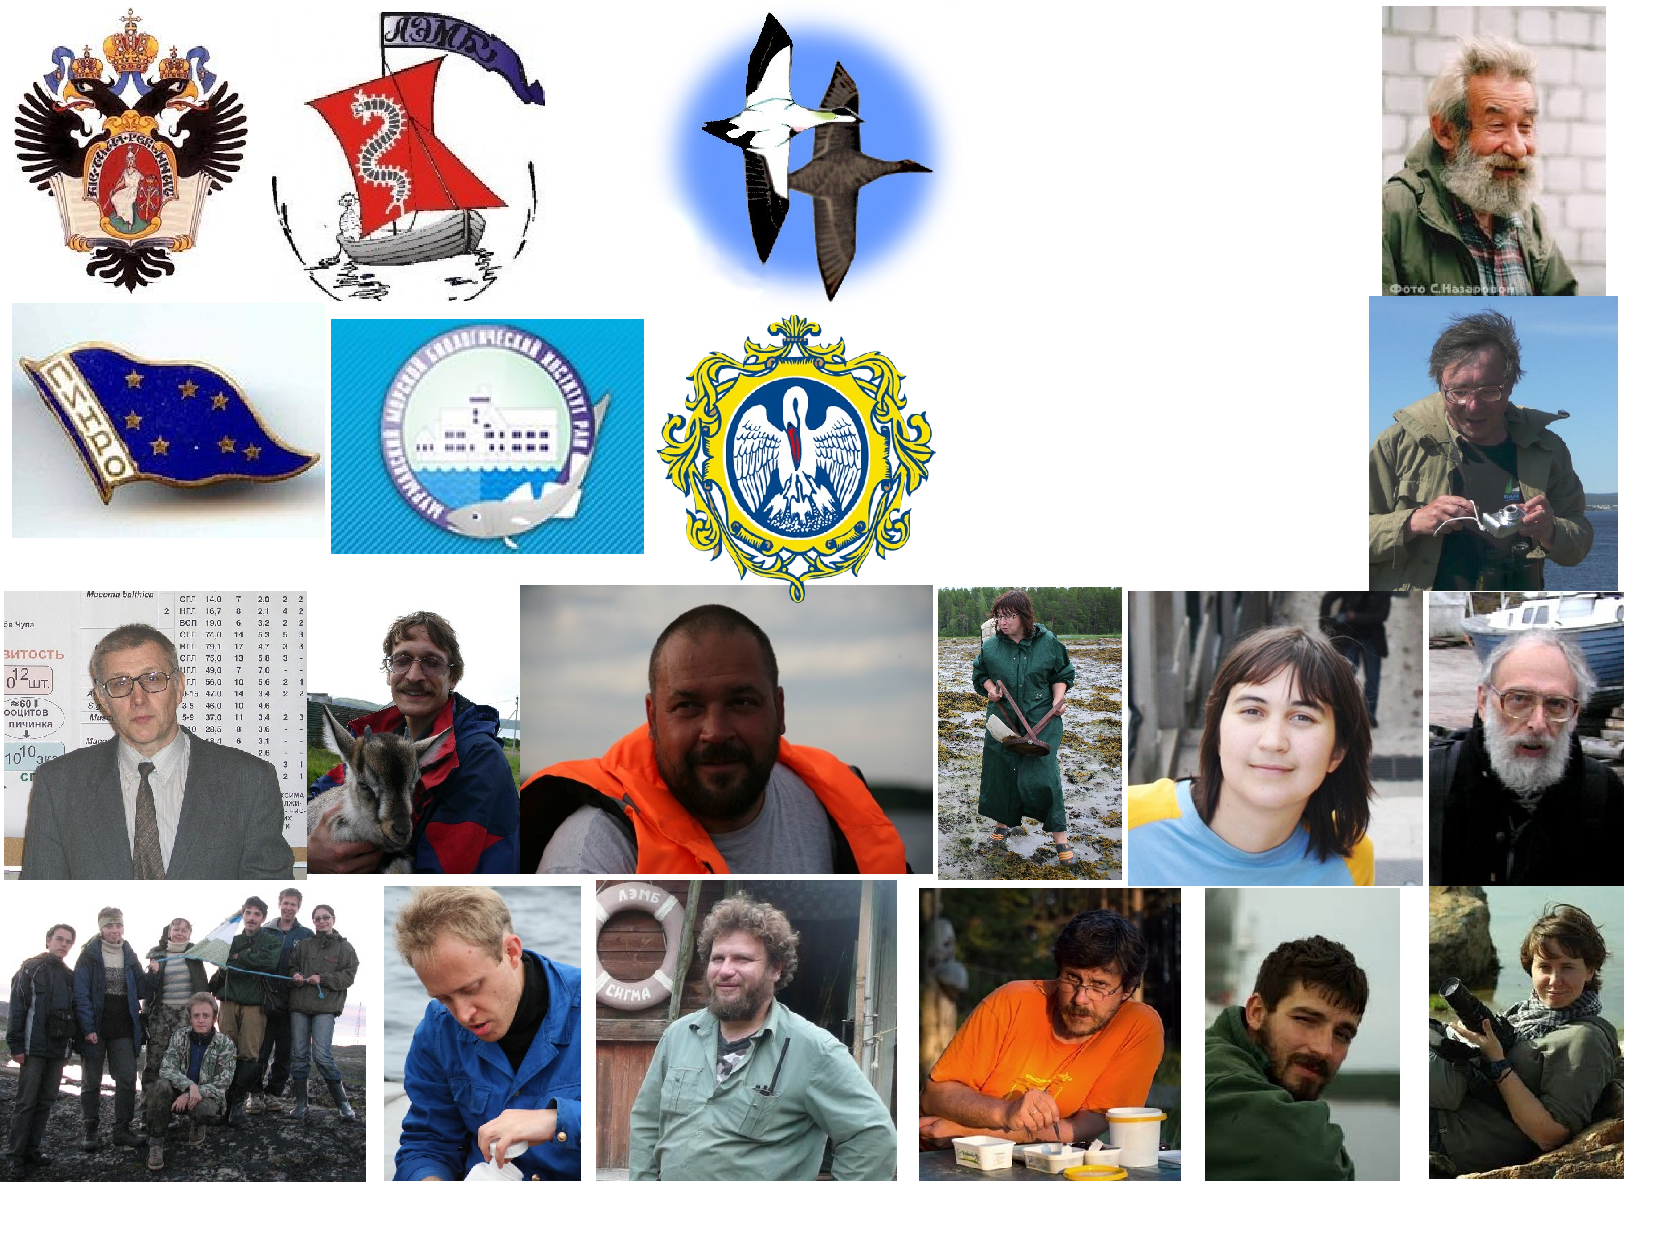
\includegraphics[height=.7\textheight]{blagodarnosti.pdf}\\
\end{center}
{\tiny Работа частично поддержана грантами СПбГУ: 1.0.134.2010, 1.42.527.2011, 1.41.862.2011, 1.42.282.2012, 1.42.514.2013, 1.38.253.2014}
\end{frame}


\end{document}
